% Cerata - IEEEtran journal paper.
% Build: cd paper && mkdir -p build && nix run nixpkgs#tectonic -- main.tex -o build
% Numbers: run `.venv/bin/python paper/make_numbers.py` from the repository root.
\documentclass[journal,10pt]{IEEEtran}

\usepackage{booktabs}
\usepackage{amsmath}
\usepackage[T1]{fontenc}
\usepackage{newtxtext,newtxmath}
\usepackage{tikz}
\usetikzlibrary{arrows.meta,positioning,shapes.geometric,calc}
\usepackage{pgfplots}
\pgfplotsset{compat=1.17}
\usepackage{graphicx}
\usepackage{xcolor}
\usepackage{array}
\usepackage{algorithm}
\usepackage{algpseudocode}
\usepackage[hidelinks]{hyperref}

\newtheorem{proposition}{Proposition}

% Abstract and index terms without the template's em dashes; no hyphenation in the
% index terms.
\makeatletter
\def\abstract{\normalfont\small\noindent\textbf{Abstract.}\enspace\@IEEEgobbleleadPARNLSP}
\def\IEEEkeywords{\normalfont\small\noindent\textbf{Index Terms.}\enspace
  \hyphenpenalty=10000\exhyphenpenalty=10000\@IEEEgobbleleadPARNLSP}
\makeatother

% All result macros are generated by make_numbers.py from the result files of
% prereg entries SS64 to SS78 (results/live_learning/confirm/).
% Generated from results/live_learning/confirm/*_n1000_routed_eval.json (prereg SS64).
\newcommand{\cfEff}{0.997}
\newcommand{\cfEffPct}{99.7}
\newcommand{\cfEffCI}{.993,1}
\newcommand{\cfPara}{0.323}
\newcommand{\cfParaPct}{32.3}
\newcommand{\cfParaCI}{.295,.352}
\newcommand{\cfNoLeak}{0.992}
\newcommand{\cfNoLeakPct}{99.2}
\newcommand{\cfNoLeakCI}{.986,.997}
\newcommand{\cfGone}{0.96}
\newcommand{\cfGonePct}{96}
\newcommand{\cfGoneCI}{.92,.99}
\newcommand{\cfReturn}{0.96}
\newcommand{\cfReturnPct}{96}
\newcommand{\cfReturnCI}{.92,.99}
\newcommand{\cfRetain}{0.997}
\newcommand{\cfRetainPct}{99.7}
\newcommand{\cfRetainCI}{.992,1}
\newcommand{\cfRoute}{0.997}
\newcommand{\cfParaRoute}{0.362}
\newcommand{\cfAbst}{0.992}
\newcommand{\cfAbstPct}{99.2}
\newcommand{\cfRoutePct}{99.7}
\newcommand{\cfRevMs}{2.6}
\newcommand{\cfEffErr}{0.004}
\newcommand{\zsEff}{0.994}
\newcommand{\zsEffPct}{99.4}
\newcommand{\zsEffCI}{.989,.998}
\newcommand{\zsPara}{0.973}
\newcommand{\zsParaPct}{97.3}
\newcommand{\zsParaCI}{.962,.982}
\newcommand{\zsNoLeak}{0.975}
\newcommand{\zsNoLeakPct}{97.5}
\newcommand{\zsNoLeakCI}{.965,.984}
\newcommand{\zsGone}{0.36}
\newcommand{\zsGonePct}{36}
\newcommand{\zsGoneCI}{.26,.45}
\newcommand{\zsReturn}{0.80}
\newcommand{\zsReturnPct}{80}
\newcommand{\zsReturnCI}{.72,.88}
\newcommand{\zsRetain}{0.992}
\newcommand{\zsRetainPct}{99.2}
\newcommand{\zsRetainCI}{.986,.998}
\newcommand{\zsRoute}{0.784}
\newcommand{\zsParaRoute}{0.776}
\newcommand{\zsAbst}{0.967}
\newcommand{\zsAbstPct}{96.7}
\newcommand{\zsRoutePct}{78.4}
\newcommand{\zsRevMs}{2.4}
\newcommand{\zsEffErr}{0.005}
\newcommand{\vCfEff}{0.997}
\newcommand{\vCfEffPct}{99.7}
\newcommand{\vCfEffCI}{.993,1}
\newcommand{\vCfEffRet}{0.838}
\newcommand{\vCfEffRetPct}{83.8}
\newcommand{\vCfEffRetCI}{.816,.86}
\newcommand{\vCfEffBoth}{0.996}
\newcommand{\vCfEffBothPct}{99.6}
\newcommand{\vCfEffBothCI}{.992,.999}
\newcommand{\vCfRoute}{0.998}
\newcommand{\vCfRoutePct}{99.8}
\newcommand{\vCfRouteCI}{.995,1}
\newcommand{\vCfPara}{0.669}
\newcommand{\vCfParaPct}{66.9}
\newcommand{\vCfParaCI}{.641,.699}
\newcommand{\vCfParaRet}{0.629}
\newcommand{\vCfParaRetPct}{62.9}
\newcommand{\vCfParaRetCI}{.601,.659}
\newcommand{\vCfParaBoth}{0.803}
\newcommand{\vCfParaBothPct}{80.3}
\newcommand{\vCfParaBothCI}{.778,.827}
\newcommand{\vCfParaRouted}{0.818}
\newcommand{\vCfParaRoutedPct}{81.8}
\newcommand{\vCfParaRoutedCI}{.794,.841}
\newcommand{\vCfParaRoute}{0.814}
\newcommand{\vCfParaRoutePct}{81.4}
\newcommand{\vCfParaRouteCI}{.789,.838}
\newcommand{\vCfParaDiff}{4.0}
\newcommand{\vCfParaDiffCI}{1.1 to 6.8}
\newcommand{\vCfEffDiff}{15.9}
\newcommand{\vCfEffDiffCI}{13.7 to 18.1}
\newcommand{\vCfNoLeak}{1.00}
\newcommand{\vCfNoLeakPct}{100}
\newcommand{\vCfNoLeakCI}{1,1}
\newcommand{\vCfTierFrac}{0.162}
\newcommand{\vCfTierFracPct}{16.2}
\newcommand{\vCfTierEff}{0.998}
\newcommand{\vCfTierEffPct}{99.8}
\newcommand{\vCfTierEffCI}{.995,1}
\newcommand{\vCfTierPara}{0.664}
\newcommand{\vCfTierParaPct}{66.4}
\newcommand{\vCfTierParaCI}{.635,.694}
\newcommand{\vCfGone}{1.00}
\newcommand{\vCfGonePct}{100}
\newcommand{\vCfGoneCI}{1,1}
\newcommand{\vCfReturn}{1.00}
\newcommand{\vCfReturnPct}{100}
\newcommand{\vCfReturnCI}{1,1}
\newcommand{\vCfRetain}{0.997}
\newcommand{\vCfRetainPct}{99.7}
\newcommand{\vCfRetainCI}{.992,1}
\newcommand{\vCfEtwoRouted}{0.018}
\newcommand{\vCfEtwoRoutedPct}{1.8}
\newcommand{\vCfEtwoRoutedCI}{.01,.027}
\newcommand{\vCfEtwoSame}{0.982}
\newcommand{\vCfEtwoSamePct}{98.2}
\newcommand{\vCfEtwoSameCI}{.973,.99}
\newcommand{\vCfEtwoLeak}{0.014}
\newcommand{\vCfEtwoLeakPct}{1.4}
\newcommand{\vCfEtwoLeakCI}{.007,.022}
\newcommand{\vCfEthreeRouted}{0.29}
\newcommand{\vCfEthreeRoutedPct}{29}
\newcommand{\vCfEthreeRoutedCI}{.263,.317}
\newcommand{\vCfEthreeSame}{0.711}
\newcommand{\vCfEthreeSamePct}{71.1}
\newcommand{\vCfEthreeSameCI}{.684,.738}
\newcommand{\vCfEthreeLeak}{0.186}
\newcommand{\vCfEthreeLeakPct}{18.6}
\newcommand{\vCfEthreeLeakCI}{.162,.209}
\newcommand{\vZsEff}{0.999}
\newcommand{\vZsEffPct}{99.9}
\newcommand{\vZsEffCI}{.997,1}
\newcommand{\vZsEffRet}{0.794}
\newcommand{\vZsEffRetPct}{79.4}
\newcommand{\vZsEffRetCI}{.768,.82}
\newcommand{\vZsEffBoth}{0.989}
\newcommand{\vZsEffBothPct}{98.9}
\newcommand{\vZsEffBothCI}{.982,.995}
\newcommand{\vZsRoute}{1.00}
\newcommand{\vZsRoutePct}{100}
\newcommand{\vZsRouteCI}{1,1}
\newcommand{\vZsPara}{0.959}
\newcommand{\vZsParaPct}{95.9}
\newcommand{\vZsParaCI}{.946,.971}
\newcommand{\vZsParaRet}{0.817}
\newcommand{\vZsParaRetPct}{81.7}
\newcommand{\vZsParaRetCI}{.792,.84}
\newcommand{\vZsParaBoth}{0.979}
\newcommand{\vZsParaBothPct}{97.9}
\newcommand{\vZsParaBothCI}{.969,.988}
\newcommand{\vZsParaRouted}{0.964}
\newcommand{\vZsParaRoutedPct}{96.4}
\newcommand{\vZsParaRoutedCI}{.952,.975}
\newcommand{\vZsParaRoute}{0.74}
\newcommand{\vZsParaRoutePct}{74}
\newcommand{\vZsParaRouteCI}{.711,.765}
\newcommand{\vZsParaDiff}{14.2}
\newcommand{\vZsParaDiffCI}{11.7 to 16.7}
\newcommand{\vZsEffDiff}{20.5}
\newcommand{\vZsEffDiffCI}{18.0 to 23.0}
\newcommand{\vZsNoLeak}{1.00}
\newcommand{\vZsNoLeakPct}{100}
\newcommand{\vZsNoLeakCI}{1,1}
\newcommand{\vZsTierFrac}{0.206}
\newcommand{\vZsTierFracPct}{20.6}
\newcommand{\vZsTierEff}{1.00}
\newcommand{\vZsTierEffPct}{100}
\newcommand{\vZsTierEffCI}{1,1}
\newcommand{\vZsTierPara}{0.931}
\newcommand{\vZsTierParaPct}{93.1}
\newcommand{\vZsTierParaCI}{.915,.946}
\newcommand{\vZsGone}{0.42}
\newcommand{\vZsGonePct}{42}
\newcommand{\vZsGoneCI}{.32,.52}
\newcommand{\vZsReturn}{0.86}
\newcommand{\vZsReturnPct}{86}
\newcommand{\vZsReturnCI}{.79,.92}
\newcommand{\vZsRetain}{0.999}
\newcommand{\vZsRetainPct}{99.9}
\newcommand{\vZsRetainCI}{.997,1}
\newcommand{\vZsReturnContent}{1.00}
\newcommand{\vZsReturnContentPct}{100}
\newcommand{\vZsReturnContentCI}{1,1}
\newcommand{\vZsContentExtra}{38}
\newcommand{\vZsLocRouted}{0.00}
\newcommand{\vZsLocRoutedPct}{0}
\newcommand{\vZsLocRoutedCI}{0,0}
\newcommand{\vZsLocSame}{1.00}
\newcommand{\vZsLocSamePct}{100}
\newcommand{\vZsLocSameCI}{1,1}
\newcommand{\vZsLocLeak}{0.00}
\newcommand{\vZsLocLeakPct}{0}
\newcommand{\vZsLocLeakCI}{0,0}
\newcommand{\chkInMean}{0.022}
\newcommand{\chkInMeanPct}{2.2}
\newcommand{\chkInMax}{0.078}
\newcommand{\chkInMaxPct}{7.8}
\newcommand{\chkHeldMean}{0.364}
\newcommand{\chkHeldMeanPct}{36.4}
\newcommand{\chkHeldMax}{1.072}
\newcommand{\chkHeldMaxPct}{107.2}
\newcommand{\chkKappa}{0.968}
\newcommand{\chkKappaPct}{96.8}
\newcommand{\chkWrongRoute}{0.72}
\newcommand{\chkWrongRoutePct}{72}
\newcommand{\vCfEthreeLeakAdapter}{0.186}
\newcommand{\vCfEthreeLeakAdapterPct}{18.6}
\newcommand{\vCfEthreeLeakAdapterCI}{.162,.209}
\newcommand{\vCfEthreeLeakNote}{0.14}
\newcommand{\vCfEthreeLeakNotePct}{14}
\newcommand{\vCfEthreeLeakNoteCI}{.118,.161}
\newcommand{\vCfEthreeLeakBoth}{0.237}
\newcommand{\vCfEthreeLeakBothPct}{23.7}
\newcommand{\vCfEthreeLeakBothCI}{.21,.262}
\newcommand{\vCfEthreeLeakTiered}{0.155}
\newcommand{\vCfEthreeLeakTieredPct}{15.5}
\newcommand{\vCfEthreeLeakTieredCI}{.133,.176}
\newcommand{\yTheta}{0.660}
\newcommand{\yCfEff}{0.997}
\newcommand{\yCfEffPct}{99.7}
\newcommand{\yCfEffRet}{0.838}
\newcommand{\yCfEffRetPct}{83.8}
\newcommand{\yCfEffBoth}{0.996}
\newcommand{\yCfEffBothPct}{99.6}
\newcommand{\yCfEffBothCI}{.992,.999}
\newcommand{\yCfEffTier}{0.998}
\newcommand{\yCfEffTierPct}{99.8}
\newcommand{\yCfEffRoute}{0.998}
\newcommand{\yCfEffRoutePct}{99.8}
\newcommand{\yCfPara}{0.643}
\newcommand{\yCfParaPct}{64.3}
\newcommand{\yCfParaRet}{0.607}
\newcommand{\yCfParaRetPct}{60.7}
\newcommand{\yCfParaBoth}{0.768}
\newcommand{\yCfParaBothPct}{76.8}
\newcommand{\yCfParaBothCI}{.742,.794}
\newcommand{\yCfParaTier}{0.642}
\newcommand{\yCfParaTierPct}{64.2}
\newcommand{\yCfParaRoute}{0.776}
\newcommand{\yCfParaRoutePct}{77.6}
\newcommand{\yZsEff}{0.999}
\newcommand{\yZsEffPct}{99.9}
\newcommand{\yZsEffRet}{0.794}
\newcommand{\yZsEffRetPct}{79.4}
\newcommand{\yZsEffBoth}{0.989}
\newcommand{\yZsEffBothPct}{98.9}
\newcommand{\yZsEffBothCI}{.982,.995}
\newcommand{\yZsEffTier}{1.00}
\newcommand{\yZsEffTierPct}{100}
\newcommand{\yZsEffRoute}{1.00}
\newcommand{\yZsEffRoutePct}{100}
\newcommand{\yZsPara}{0.955}
\newcommand{\yZsParaPct}{95.5}
\newcommand{\yZsParaRet}{0.816}
\newcommand{\yZsParaRetPct}{81.6}
\newcommand{\yZsParaBoth}{0.975}
\newcommand{\yZsParaBothPct}{97.5}
\newcommand{\yZsParaBothCI}{.965,.984}
\newcommand{\yZsParaTier}{0.929}
\newcommand{\yZsParaTierPct}{92.9}
\newcommand{\yZsParaRoute}{0.729}
\newcommand{\yZsParaRoutePct}{72.9}
\newcommand{\yCfEthreeRouted}{0.207}
\newcommand{\yCfEthreeRoutedPct}{20.7}
\newcommand{\yCfEthreeLeakAdapter}{0.14}
\newcommand{\yCfEthreeLeakAdapterPct}{14}
\newcommand{\yCfEthreeLeakAdapterCI}{.119,.16}
\newcommand{\yCfEthreeLeakNote}{0.109}
\newcommand{\yCfEthreeLeakNotePct}{10.9}
\newcommand{\yCfEthreeLeakNoteCI}{.089,.128}
\newcommand{\yCfEthreeLeakBoth}{0.171}
\newcommand{\yCfEthreeLeakBothPct}{17.1}
\newcommand{\yCfEthreeLeakBothCI}{.147,.194}
\newcommand{\yCfEthreeLeakTiered}{0.121}
\newcommand{\yCfEthreeLeakTieredPct}{12.1}
\newcommand{\yCfEthreeLeakTieredCI}{.101,.14}
\newcommand{\yCfEtwoRouted}{0.017}
\newcommand{\yCfEtwoRoutedPct}{1.7}
\newcommand{\yCfEtwoLeakAdapter}{0.014}
\newcommand{\yCfEtwoLeakAdapterPct}{1.4}
\newcommand{\yCfEtwoLeakAdapterCI}{.007,.022}
\newcommand{\yCfEtwoLeakNote}{0.013}
\newcommand{\yCfEtwoLeakNotePct}{1.3}
\newcommand{\yCfEtwoLeakNoteCI}{.007,.02}
\newcommand{\yCfEtwoLeakBoth}{0.015}
\newcommand{\yCfEtwoLeakBothPct}{1.5}
\newcommand{\yCfEtwoLeakBothCI}{.008,.023}
\newcommand{\yCfEtwoLeakTiered}{0.014}
\newcommand{\yCfEtwoLeakTieredPct}{1.4}
\newcommand{\yCfEtwoLeakTieredCI}{.007,.022}
\newcommand{\sTheta}{0.757}
\newcommand{\sCfEff}{0.997}
\newcommand{\sCfEffPct}{99.7}
\newcommand{\sCfEffRet}{0.838}
\newcommand{\sCfEffRetPct}{83.8}
\newcommand{\sCfEffBoth}{0.996}
\newcommand{\sCfEffBothPct}{99.6}
\newcommand{\sCfEffBothCI}{.992,.999}
\newcommand{\sCfEffTier}{0.998}
\newcommand{\sCfEffTierPct}{99.8}
\newcommand{\sCfEffRoute}{0.998}
\newcommand{\sCfEffRoutePct}{99.8}
\newcommand{\sCfPara}{0.513}
\newcommand{\sCfParaPct}{51.3}
\newcommand{\sCfParaRet}{0.488}
\newcommand{\sCfParaRetPct}{48.8}
\newcommand{\sCfParaBoth}{0.589}
\newcommand{\sCfParaBothPct}{58.9}
\newcommand{\sCfParaBothCI}{.559,.618}
\newcommand{\sCfParaTier}{0.512}
\newcommand{\sCfParaTierPct}{51.2}
\newcommand{\sCfParaRoute}{0.595}
\newcommand{\sCfParaRoutePct}{59.5}
\newcommand{\sZsEff}{0.999}
\newcommand{\sZsEffPct}{99.9}
\newcommand{\sZsEffRet}{0.794}
\newcommand{\sZsEffRetPct}{79.4}
\newcommand{\sZsEffBoth}{0.989}
\newcommand{\sZsEffBothPct}{98.9}
\newcommand{\sZsEffBothCI}{.982,.995}
\newcommand{\sZsEffTier}{1.00}
\newcommand{\sZsEffTierPct}{100}
\newcommand{\sZsEffRoute}{1.00}
\newcommand{\sZsEffRoutePct}{100}
\newcommand{\sZsPara}{0.938}
\newcommand{\sZsParaPct}{93.8}
\newcommand{\sZsParaRet}{0.807}
\newcommand{\sZsParaRetPct}{80.7}
\newcommand{\sZsParaBoth}{0.956}
\newcommand{\sZsParaBothPct}{95.6}
\newcommand{\sZsParaBothCI}{.943,.968}
\newcommand{\sZsParaTier}{0.914}
\newcommand{\sZsParaTierPct}{91.4}
\newcommand{\sZsParaRoute}{0.694}
\newcommand{\sZsParaRoutePct}{69.4}
\newcommand{\sCfEthreeRouted}{0.064}
\newcommand{\sCfEthreeRoutedPct}{6.4}
\newcommand{\sCfEthreeLeakAdapter}{0.058}
\newcommand{\sCfEthreeLeakAdapterPct}{5.8}
\newcommand{\sCfEthreeLeakAdapterCI}{.044,.072}
\newcommand{\sCfEthreeLeakNote}{0.045}
\newcommand{\sCfEthreeLeakNotePct}{4.5}
\newcommand{\sCfEthreeLeakNoteCI}{.033,.058}
\newcommand{\sCfEthreeLeakBoth}{0.063}
\newcommand{\sCfEthreeLeakBothPct}{6.3}
\newcommand{\sCfEthreeLeakBothCI}{.048,.078}
\newcommand{\sCfEthreeLeakTiered}{0.053}
\newcommand{\sCfEthreeLeakTieredPct}{5.3}
\newcommand{\sCfEthreeLeakTieredCI}{.039,.067}
\newcommand{\sCfEtwoRouted}{0.012}
\newcommand{\sCfEtwoRoutedPct}{1.2}
\newcommand{\sCfEtwoLeakAdapter}{0.011}
\newcommand{\sCfEtwoLeakAdapterPct}{1.1}
\newcommand{\sCfEtwoLeakAdapterCI}{.005,.018}
\newcommand{\sCfEtwoLeakNote}{0.009}
\newcommand{\sCfEtwoLeakNotePct}{0.9}
\newcommand{\sCfEtwoLeakNoteCI}{.004,.016}
\newcommand{\sCfEtwoLeakBoth}{0.011}
\newcommand{\sCfEtwoLeakBothPct}{1.1}
\newcommand{\sCfEtwoLeakBothCI}{.005,.018}
\newcommand{\sCfEtwoLeakTiered}{0.01}
\newcommand{\sCfEtwoLeakTieredPct}{1}
\newcommand{\sCfEtwoLeakTieredCI}{.004,.017}
\newcommand{\aucRelCf}{0.790}
\newcommand{\aucRelPool}{0.848}
\newcommand{\aucJudgeCf}{0.775}
\newcommand{\aucJudgePool}{0.827}
\newcommand{\aucTypeCf}{0.649}
\newcommand{\aucTypePool}{0.646}
\newcommand{\wCfEff}{0.997}
\newcommand{\wCfEffPct}{99.7}
\newcommand{\wCfEffCI}{.993,1}
\newcommand{\wCfEffCIPct}{99.3 to 100.0}
\newcommand{\wCfEffRet}{0.838}
\newcommand{\wCfEffRetPct}{83.8}
\newcommand{\wCfEffRetCI}{.816,.86}
\newcommand{\wCfEffRetCIPct}{81.6 to 86.0}
\newcommand{\wCfEffBoth}{0.996}
\newcommand{\wCfEffBothPct}{99.6}
\newcommand{\wCfEffBothCI}{.992,.999}
\newcommand{\wCfEffBothCIPct}{99.2 to 99.9}
\newcommand{\wCfEffRoute}{0.998}
\newcommand{\wCfEffRoutePct}{99.8}
\newcommand{\wCfEffRouteCI}{.995,1}
\newcommand{\wCfEffRouteCIPct}{99.5 to 100.0}
\newcommand{\wCfPara}{0.530}
\newcommand{\wCfParaPct}{53.0}
\newcommand{\wCfParaCI}{.5,.561}
\newcommand{\wCfParaCIPct}{50.0 to 56.1}
\newcommand{\wCfParaRet}{0.507}
\newcommand{\wCfParaRetPct}{50.7}
\newcommand{\wCfParaRetCI}{.477,.538}
\newcommand{\wCfParaRetCIPct}{47.7 to 53.8}
\newcommand{\wCfParaBoth}{0.620}
\newcommand{\wCfParaBothPct}{62.0}
\newcommand{\wCfParaBothCI}{.591,.649}
\newcommand{\wCfParaBothCIPct}{59.1 to 64.9}
\newcommand{\wCfParaRoute}{0.623}
\newcommand{\wCfParaRoutePct}{62.3}
\newcommand{\wCfParaRouteCI}{.593,.652}
\newcommand{\wCfParaRouteCIPct}{59.3 to 65.2}
\newcommand{\wCfParaTier}{0.525}
\newcommand{\wCfParaTierPct}{52.5}
\newcommand{\wCfParaTierCI}{.494,.555}
\newcommand{\wCfParaTierCIPct}{49.4 to 55.5}
\newcommand{\wCfTierFrac}{0.162}
\newcommand{\wCfTierFracPct}{16.2}
\newcommand{\wCfReturn}{1.000}
\newcommand{\wCfReturnPct}{100.0}
\newcommand{\wCfReturnCI}{1,1}
\newcommand{\wCfReturnCIPct}{100.0 to 100.0}
\newcommand{\wCfRetain}{0.997}
\newcommand{\wCfRetainPct}{99.7}
\newcommand{\wCfRetainCI}{.992,1}
\newcommand{\wCfRetainCIPct}{99.2 to 100.0}
\newcommand{\wCfNoLeak}{1.000}
\newcommand{\wCfNoLeakPct}{100.0}
\newcommand{\wCfNoLeakCI}{1,1}
\newcommand{\wCfNoLeakCIPct}{100.0 to 100.0}
\newcommand{\wCfEthreeRouted}{0.057}
\newcommand{\wCfEthreeRoutedPct}{5.7}
\newcommand{\wCfEthreeRoutedCI}{.043,.07}
\newcommand{\wCfEthreeRoutedCIPct}{4.3 to 7.0}
\newcommand{\wCfEthreeLeakAdapter}{0.050}
\newcommand{\wCfEthreeLeakAdapterPct}{5.0}
\newcommand{\wCfEthreeLeakAdapterCI}{.037,.063}
\newcommand{\wCfEthreeLeakAdapterCIPct}{3.7 to 6.3}
\newcommand{\wCfEthreeLeakNote}{0.038}
\newcommand{\wCfEthreeLeakNotePct}{3.8}
\newcommand{\wCfEthreeLeakNoteCI}{.026,.05}
\newcommand{\wCfEthreeLeakNoteCIPct}{2.6 to 5.0}
\newcommand{\wCfEthreeLeakBoth}{0.050}
\newcommand{\wCfEthreeLeakBothPct}{5.0}
\newcommand{\wCfEthreeLeakBothCI}{.037,.063}
\newcommand{\wCfEthreeLeakBothCIPct}{3.7 to 6.3}
\newcommand{\wCfEthreeLeakTiered}{0.043}
\newcommand{\wCfEthreeLeakTieredPct}{4.3}
\newcommand{\wCfEthreeLeakTieredCI}{.031,.055}
\newcommand{\wCfEthreeLeakTieredCIPct}{3.1 to 5.5}
\newcommand{\wCfEtwoRouted}{0.010}
\newcommand{\wCfEtwoRoutedPct}{1.0}
\newcommand{\wCfEtwoRoutedCI}{.004,.016}
\newcommand{\wCfEtwoRoutedCIPct}{0.4 to 1.6}
\newcommand{\wCfEtwoLeakAdapter}{0.009}
\newcommand{\wCfEtwoLeakAdapterPct}{0.9}
\newcommand{\wCfEtwoLeakAdapterCI}{.004,.015}
\newcommand{\wCfEtwoLeakAdapterCIPct}{0.4 to 1.5}
\newcommand{\wCfEtwoLeakNote}{0.008}
\newcommand{\wCfEtwoLeakNotePct}{0.8}
\newcommand{\wCfEtwoLeakNoteCI}{.003,.014}
\newcommand{\wCfEtwoLeakNoteCIPct}{0.3 to 1.4}
\newcommand{\wCfEtwoLeakBoth}{0.009}
\newcommand{\wCfEtwoLeakBothPct}{0.9}
\newcommand{\wCfEtwoLeakBothCI}{.004,.015}
\newcommand{\wCfEtwoLeakBothCIPct}{0.4 to 1.5}
\newcommand{\wCfEtwoLeakTiered}{0.009}
\newcommand{\wCfEtwoLeakTieredPct}{0.9}
\newcommand{\wCfEtwoLeakTieredCI}{.004,.015}
\newcommand{\wCfEtwoLeakTieredCIPct}{0.4 to 1.5}
\newcommand{\wZsEff}{0.999}
\newcommand{\wZsEffPct}{99.9}
\newcommand{\wZsEffCI}{.997,1}
\newcommand{\wZsEffCIPct}{99.7 to 100.0}
\newcommand{\wZsEffRet}{0.794}
\newcommand{\wZsEffRetPct}{79.4}
\newcommand{\wZsEffRetCI}{.768,.82}
\newcommand{\wZsEffRetCIPct}{76.8 to 82.0}
\newcommand{\wZsEffBoth}{0.989}
\newcommand{\wZsEffBothPct}{98.9}
\newcommand{\wZsEffBothCI}{.982,.995}
\newcommand{\wZsEffBothCIPct}{98.2 to 99.5}
\newcommand{\wZsEffRoute}{0.997}
\newcommand{\wZsEffRoutePct}{99.7}
\newcommand{\wZsEffRouteCI}{.993,1}
\newcommand{\wZsEffRouteCIPct}{99.3 to 100.0}
\newcommand{\wZsPara}{0.947}
\newcommand{\wZsParaPct}{94.7}
\newcommand{\wZsParaCI}{.932,.96}
\newcommand{\wZsParaCIPct}{93.2 to 96.0}
\newcommand{\wZsParaRet}{0.804}
\newcommand{\wZsParaRetPct}{80.4}
\newcommand{\wZsParaRetCI}{.78,.828}
\newcommand{\wZsParaRetCIPct}{78.0 to 82.8}
\newcommand{\wZsParaBoth}{0.960}
\newcommand{\wZsParaBothPct}{96.0}
\newcommand{\wZsParaBothCI}{.948,.972}
\newcommand{\wZsParaBothCIPct}{94.8 to 97.2}
\newcommand{\wZsParaRoute}{0.721}
\newcommand{\wZsParaRoutePct}{72.1}
\newcommand{\wZsParaRouteCI}{.693,.748}
\newcommand{\wZsParaRouteCIPct}{69.3 to 74.8}
\newcommand{\wZsParaTier}{0.918}
\newcommand{\wZsParaTierPct}{91.8}
\newcommand{\wZsParaTierCI}{.901,.934}
\newcommand{\wZsParaTierCIPct}{90.1 to 93.4}
\newcommand{\wZsTierFrac}{0.206}
\newcommand{\wZsTierFracPct}{20.6}
\newcommand{\wZsReturn}{0.880}
\newcommand{\wZsReturnPct}{88.0}
\newcommand{\wZsReturnCI}{.81,.94}
\newcommand{\wZsReturnCIPct}{81.0 to 94.0}
\newcommand{\wZsRetain}{0.999}
\newcommand{\wZsRetainPct}{99.9}
\newcommand{\wZsRetainCI}{.997,1}
\newcommand{\wZsRetainCIPct}{99.7 to 100.0}
\newcommand{\wZsNoLeak}{1.000}
\newcommand{\wZsNoLeakPct}{100.0}
\newcommand{\wZsNoLeakCI}{1,1}
\newcommand{\wZsNoLeakCIPct}{100.0 to 100.0}
\newcommand{\wZsLocRouted}{0.000}
\newcommand{\wZsLocRoutedPct}{0.0}
\newcommand{\wZsLocRoutedCI}{0,0}
\newcommand{\wZsLocRoutedCIPct}{0.0 to 0.0}
\newcommand{\wZsLocLeakAdapter}{0.000}
\newcommand{\wZsLocLeakAdapterPct}{0.0}
\newcommand{\wZsLocLeakAdapterCI}{0,0}
\newcommand{\wZsLocLeakAdapterCIPct}{0.0 to 0.0}
\newcommand{\wZsLocLeakNote}{0.000}
\newcommand{\wZsLocLeakNotePct}{0.0}
\newcommand{\wZsLocLeakNoteCI}{0,0}
\newcommand{\wZsLocLeakNoteCIPct}{0.0 to 0.0}
\newcommand{\wZsLocLeakBoth}{0.000}
\newcommand{\wZsLocLeakBothPct}{0.0}
\newcommand{\wZsLocLeakBothCI}{0,0}
\newcommand{\wZsLocLeakBothCIPct}{0.0 to 0.0}
\newcommand{\wZsLocLeakTiered}{0.000}
\newcommand{\wZsLocLeakTieredPct}{0.0}
\newcommand{\wZsLocLeakTieredCI}{0,0}
\newcommand{\wZsLocLeakTieredCIPct}{0.0 to 0.0}
\newcommand{\xCfEff}{0.997}
\newcommand{\xCfEffPct}{99.7}
\newcommand{\xCfEffCI}{.993,1}
\newcommand{\xCfEffCIPct}{99.3 to 100.0}
\newcommand{\xCfEffRet}{0.838}
\newcommand{\xCfEffRetPct}{83.8}
\newcommand{\xCfEffRetCI}{.816,.86}
\newcommand{\xCfEffRetCIPct}{81.6 to 86.0}
\newcommand{\xCfEffBoth}{0.996}
\newcommand{\xCfEffBothPct}{99.6}
\newcommand{\xCfEffBothCI}{.992,.999}
\newcommand{\xCfEffBothCIPct}{99.2 to 99.9}
\newcommand{\xCfEffRoute}{0.998}
\newcommand{\xCfEffRoutePct}{99.8}
\newcommand{\xCfEffRouteCI}{.995,1}
\newcommand{\xCfEffRouteCIPct}{99.5 to 100.0}
\newcommand{\xCfPara}{0.730}
\newcommand{\xCfParaPct}{73.0}
\newcommand{\xCfParaCI}{.704,.757}
\newcommand{\xCfParaCIPct}{70.4 to 75.7}
\newcommand{\xCfParaRet}{0.684}
\newcommand{\xCfParaRetPct}{68.4}
\newcommand{\xCfParaRetCI}{.656,.713}
\newcommand{\xCfParaRetCIPct}{65.6 to 71.3}
\newcommand{\xCfParaBoth}{0.891}
\newcommand{\xCfParaBothPct}{89.1}
\newcommand{\xCfParaBothCI}{.872,.91}
\newcommand{\xCfParaBothCIPct}{87.2 to 91.0}
\newcommand{\xCfParaRoute}{0.908}
\newcommand{\xCfParaRoutePct}{90.8}
\newcommand{\xCfParaRouteCI}{.89,.925}
\newcommand{\xCfParaRouteCIPct}{89.0 to 92.5}
\newcommand{\xCfParaTier}{0.723}
\newcommand{\xCfParaTierPct}{72.3}
\newcommand{\xCfParaTierCI}{.697,.751}
\newcommand{\xCfParaTierCIPct}{69.7 to 75.1}
\newcommand{\xCfTierFrac}{0.162}
\newcommand{\xCfTierFracPct}{16.2}
\newcommand{\xCfReturn}{1.000}
\newcommand{\xCfReturnPct}{100.0}
\newcommand{\xCfReturnCI}{1,1}
\newcommand{\xCfReturnCIPct}{100.0 to 100.0}
\newcommand{\xCfRetain}{0.997}
\newcommand{\xCfRetainPct}{99.7}
\newcommand{\xCfRetainCI}{.992,1}
\newcommand{\xCfRetainCIPct}{99.2 to 100.0}
\newcommand{\xCfNoLeak}{1.000}
\newcommand{\xCfNoLeakPct}{100.0}
\newcommand{\xCfNoLeakCI}{1,1}
\newcommand{\xCfNoLeakCIPct}{100.0 to 100.0}
\newcommand{\xCfEthreeRouted}{0.044}
\newcommand{\xCfEthreeRoutedPct}{4.4}
\newcommand{\xCfEthreeRoutedCI}{.032,.057}
\newcommand{\xCfEthreeRoutedCIPct}{3.2 to 5.7}
\newcommand{\xCfEthreeLeakAdapter}{0.042}
\newcommand{\xCfEthreeLeakAdapterPct}{4.2}
\newcommand{\xCfEthreeLeakAdapterCI}{.03,.055}
\newcommand{\xCfEthreeLeakAdapterCIPct}{3.0 to 5.5}
\newcommand{\xCfEthreeLeakNote}{0.031}
\newcommand{\xCfEthreeLeakNotePct}{3.1}
\newcommand{\xCfEthreeLeakNoteCI}{.021,.042}
\newcommand{\xCfEthreeLeakNoteCIPct}{2.1 to 4.2}
\newcommand{\xCfEthreeLeakBoth}{0.043}
\newcommand{\xCfEthreeLeakBothPct}{4.3}
\newcommand{\xCfEthreeLeakBothCI}{.031,.056}
\newcommand{\xCfEthreeLeakBothCIPct}{3.1 to 5.6}
\newcommand{\xCfEthreeLeakTiered}{0.036}
\newcommand{\xCfEthreeLeakTieredPct}{3.6}
\newcommand{\xCfEthreeLeakTieredCI}{.025,.047}
\newcommand{\xCfEthreeLeakTieredCIPct}{2.5 to 4.7}
\newcommand{\xCfEtwoRouted}{0.018}
\newcommand{\xCfEtwoRoutedPct}{1.8}
\newcommand{\xCfEtwoRoutedCI}{.01,.027}
\newcommand{\xCfEtwoRoutedCIPct}{1.0 to 2.7}
\newcommand{\xCfEtwoLeakAdapter}{0.015}
\newcommand{\xCfEtwoLeakAdapterPct}{1.5}
\newcommand{\xCfEtwoLeakAdapterCI}{.008,.023}
\newcommand{\xCfEtwoLeakAdapterCIPct}{0.8 to 2.3}
\newcommand{\xCfEtwoLeakNote}{0.012}
\newcommand{\xCfEtwoLeakNotePct}{1.2}
\newcommand{\xCfEtwoLeakNoteCI}{.006,.02}
\newcommand{\xCfEtwoLeakNoteCIPct}{0.6 to 2.0}
\newcommand{\xCfEtwoLeakBoth}{0.017}
\newcommand{\xCfEtwoLeakBothPct}{1.7}
\newcommand{\xCfEtwoLeakBothCI}{.01,.026}
\newcommand{\xCfEtwoLeakBothCIPct}{1.0 to 2.6}
\newcommand{\xCfEtwoLeakTiered}{0.014}
\newcommand{\xCfEtwoLeakTieredPct}{1.4}
\newcommand{\xCfEtwoLeakTieredCI}{.007,.022}
\newcommand{\xCfEtwoLeakTieredCIPct}{0.7 to 2.2}
\newcommand{\xZsEff}{0.999}
\newcommand{\xZsEffPct}{99.9}
\newcommand{\xZsEffCI}{.997,1}
\newcommand{\xZsEffCIPct}{99.7 to 100.0}
\newcommand{\xZsEffRet}{0.794}
\newcommand{\xZsEffRetPct}{79.4}
\newcommand{\xZsEffRetCI}{.768,.82}
\newcommand{\xZsEffRetCIPct}{76.8 to 82.0}
\newcommand{\xZsEffBoth}{0.989}
\newcommand{\xZsEffBothPct}{98.9}
\newcommand{\xZsEffBothCI}{.982,.995}
\newcommand{\xZsEffBothCIPct}{98.2 to 99.5}
\newcommand{\xZsEffRoute}{1.000}
\newcommand{\xZsEffRoutePct}{100.0}
\newcommand{\xZsEffRouteCI}{1,1}
\newcommand{\xZsEffRouteCIPct}{100.0 to 100.0}
\newcommand{\xZsPara}{0.967}
\newcommand{\xZsParaPct}{96.7}
\newcommand{\xZsParaCI}{.955,.978}
\newcommand{\xZsParaCIPct}{95.5 to 97.8}
\newcommand{\xZsParaRet}{0.815}
\newcommand{\xZsParaRetPct}{81.5}
\newcommand{\xZsParaRetCI}{.791,.839}
\newcommand{\xZsParaRetCIPct}{79.1 to 83.9}
\newcommand{\xZsParaBoth}{0.982}
\newcommand{\xZsParaBothPct}{98.2}
\newcommand{\xZsParaBothCI}{.973,.99}
\newcommand{\xZsParaBothCIPct}{97.3 to 99.0}
\newcommand{\xZsParaRoute}{0.745}
\newcommand{\xZsParaRoutePct}{74.5}
\newcommand{\xZsParaRouteCI}{.717,.772}
\newcommand{\xZsParaRouteCIPct}{71.7 to 77.2}
\newcommand{\xZsParaTier}{0.932}
\newcommand{\xZsParaTierPct}{93.2}
\newcommand{\xZsParaTierCI}{.916,.947}
\newcommand{\xZsParaTierCIPct}{91.6 to 94.7}
\newcommand{\xZsTierFrac}{0.206}
\newcommand{\xZsTierFracPct}{20.6}
\newcommand{\xZsReturn}{0.840}
\newcommand{\xZsReturnPct}{84.0}
\newcommand{\xZsReturnCI}{.77,.91}
\newcommand{\xZsReturnCIPct}{77.0 to 91.0}
\newcommand{\xZsRetain}{0.999}
\newcommand{\xZsRetainPct}{99.9}
\newcommand{\xZsRetainCI}{.997,1}
\newcommand{\xZsRetainCIPct}{99.7 to 100.0}
\newcommand{\xZsNoLeak}{1.000}
\newcommand{\xZsNoLeakPct}{100.0}
\newcommand{\xZsNoLeakCI}{1,1}
\newcommand{\xZsNoLeakCIPct}{100.0 to 100.0}
\newcommand{\xZsLocRouted}{0.000}
\newcommand{\xZsLocRoutedPct}{0.0}
\newcommand{\xZsLocRoutedCI}{0,0}
\newcommand{\xZsLocRoutedCIPct}{0.0 to 0.0}
\newcommand{\xZsLocLeakAdapter}{0.000}
\newcommand{\xZsLocLeakAdapterPct}{0.0}
\newcommand{\xZsLocLeakAdapterCI}{0,0}
\newcommand{\xZsLocLeakAdapterCIPct}{0.0 to 0.0}
\newcommand{\xZsLocLeakNote}{0.000}
\newcommand{\xZsLocLeakNotePct}{0.0}
\newcommand{\xZsLocLeakNoteCI}{0,0}
\newcommand{\xZsLocLeakNoteCIPct}{0.0 to 0.0}
\newcommand{\xZsLocLeakBoth}{0.000}
\newcommand{\xZsLocLeakBothPct}{0.0}
\newcommand{\xZsLocLeakBothCI}{0,0}
\newcommand{\xZsLocLeakBothCIPct}{0.0 to 0.0}
\newcommand{\xZsLocLeakTiered}{0.000}
\newcommand{\xZsLocLeakTieredPct}{0.0}
\newcommand{\xZsLocLeakTieredCI}{0,0}
\newcommand{\xZsLocLeakTieredCIPct}{0.0 to 0.0}
\newcommand{\uCfEff}{0.997}
\newcommand{\uCfEffPct}{99.7}
\newcommand{\uCfEffCI}{.993,1}
\newcommand{\uCfEffCIPct}{99.3 to 100.0}
\newcommand{\uCfEffRet}{0.838}
\newcommand{\uCfEffRetPct}{83.8}
\newcommand{\uCfEffRetCI}{.816,.86}
\newcommand{\uCfEffRetCIPct}{81.6 to 86.0}
\newcommand{\uCfEffBoth}{0.996}
\newcommand{\uCfEffBothPct}{99.6}
\newcommand{\uCfEffBothCI}{.992,.999}
\newcommand{\uCfEffBothCIPct}{99.2 to 99.9}
\newcommand{\uCfEffRoute}{0.998}
\newcommand{\uCfEffRoutePct}{99.8}
\newcommand{\uCfEffRouteCI}{.995,1}
\newcommand{\uCfEffRouteCIPct}{99.5 to 100.0}
\newcommand{\uCfPara}{0.731}
\newcommand{\uCfParaPct}{73.1}
\newcommand{\uCfParaCI}{.705,.758}
\newcommand{\uCfParaCIPct}{70.5 to 75.8}
\newcommand{\uCfParaRet}{0.686}
\newcommand{\uCfParaRetPct}{68.6}
\newcommand{\uCfParaRetCI}{.659,.715}
\newcommand{\uCfParaRetCIPct}{65.9 to 71.5}
\newcommand{\uCfParaBoth}{0.890}
\newcommand{\uCfParaBothPct}{89.0}
\newcommand{\uCfParaBothCI}{.87,.909}
\newcommand{\uCfParaBothCIPct}{87.0 to 90.9}
\newcommand{\uCfParaRoute}{0.909}
\newcommand{\uCfParaRoutePct}{90.9}
\newcommand{\uCfParaRouteCI}{.891,.926}
\newcommand{\uCfParaRouteCIPct}{89.1 to 92.6}
\newcommand{\uCfParaTier}{0.725}
\newcommand{\uCfParaTierPct}{72.5}
\newcommand{\uCfParaTierCI}{.698,.752}
\newcommand{\uCfParaTierCIPct}{69.8 to 75.2}
\newcommand{\uCfTierFrac}{0.162}
\newcommand{\uCfTierFracPct}{16.2}
\newcommand{\uCfReturn}{1.000}
\newcommand{\uCfReturnPct}{100.0}
\newcommand{\uCfReturnCI}{1,1}
\newcommand{\uCfReturnCIPct}{100.0 to 100.0}
\newcommand{\uCfRetain}{0.997}
\newcommand{\uCfRetainPct}{99.7}
\newcommand{\uCfRetainCI}{.992,1}
\newcommand{\uCfRetainCIPct}{99.2 to 100.0}
\newcommand{\uCfNoLeak}{1.000}
\newcommand{\uCfNoLeakPct}{100.0}
\newcommand{\uCfNoLeakCI}{1,1}
\newcommand{\uCfNoLeakCIPct}{100.0 to 100.0}
\newcommand{\uCfEthreeRouted}{0.048}
\newcommand{\uCfEthreeRoutedPct}{4.8}
\newcommand{\uCfEthreeRoutedCI}{.035,.061}
\newcommand{\uCfEthreeRoutedCIPct}{3.5 to 6.1}
\newcommand{\uCfEthreeLeakAdapter}{0.042}
\newcommand{\uCfEthreeLeakAdapterPct}{4.2}
\newcommand{\uCfEthreeLeakAdapterCI}{.03,.054}
\newcommand{\uCfEthreeLeakAdapterCIPct}{3.0 to 5.4}
\newcommand{\uCfEthreeLeakNote}{0.033}
\newcommand{\uCfEthreeLeakNotePct}{3.3}
\newcommand{\uCfEthreeLeakNoteCI}{.022,.044}
\newcommand{\uCfEthreeLeakNoteCIPct}{2.2 to 4.4}
\newcommand{\uCfEthreeLeakBoth}{0.047}
\newcommand{\uCfEthreeLeakBothPct}{4.7}
\newcommand{\uCfEthreeLeakBothCI}{.034,.06}
\newcommand{\uCfEthreeLeakBothCIPct}{3.4 to 6.0}
\newcommand{\uCfEthreeLeakTiered}{0.037}
\newcommand{\uCfEthreeLeakTieredPct}{3.7}
\newcommand{\uCfEthreeLeakTieredCI}{.026,.048}
\newcommand{\uCfEthreeLeakTieredCIPct}{2.6 to 4.8}
\newcommand{\uCfEtwoRouted}{0.017}
\newcommand{\uCfEtwoRoutedPct}{1.7}
\newcommand{\uCfEtwoRoutedCI}{.01,.026}
\newcommand{\uCfEtwoRoutedCIPct}{1.0 to 2.6}
\newcommand{\uCfEtwoLeakAdapter}{0.015}
\newcommand{\uCfEtwoLeakAdapterPct}{1.5}
\newcommand{\uCfEtwoLeakAdapterCI}{.008,.023}
\newcommand{\uCfEtwoLeakAdapterCIPct}{0.8 to 2.3}
\newcommand{\uCfEtwoLeakNote}{0.011}
\newcommand{\uCfEtwoLeakNotePct}{1.1}
\newcommand{\uCfEtwoLeakNoteCI}{.005,.018}
\newcommand{\uCfEtwoLeakNoteCIPct}{0.5 to 1.8}
\newcommand{\uCfEtwoLeakBoth}{0.016}
\newcommand{\uCfEtwoLeakBothPct}{1.6}
\newcommand{\uCfEtwoLeakBothCI}{.009,.024}
\newcommand{\uCfEtwoLeakBothCIPct}{0.9 to 2.4}
\newcommand{\uCfEtwoLeakTiered}{0.013}
\newcommand{\uCfEtwoLeakTieredPct}{1.3}
\newcommand{\uCfEtwoLeakTieredCI}{.007,.021}
\newcommand{\uCfEtwoLeakTieredCIPct}{0.7 to 2.1}
\newcommand{\uZsEff}{0.999}
\newcommand{\uZsEffPct}{99.9}
\newcommand{\uZsEffCI}{.997,1}
\newcommand{\uZsEffCIPct}{99.7 to 100.0}
\newcommand{\uZsEffRet}{0.794}
\newcommand{\uZsEffRetPct}{79.4}
\newcommand{\uZsEffRetCI}{.768,.82}
\newcommand{\uZsEffRetCIPct}{76.8 to 82.0}
\newcommand{\uZsEffBoth}{0.989}
\newcommand{\uZsEffBothPct}{98.9}
\newcommand{\uZsEffBothCI}{.982,.995}
\newcommand{\uZsEffBothCIPct}{98.2 to 99.5}
\newcommand{\uZsEffRoute}{1.000}
\newcommand{\uZsEffRoutePct}{100.0}
\newcommand{\uZsEffRouteCI}{1,1}
\newcommand{\uZsEffRouteCIPct}{100.0 to 100.0}
\newcommand{\uZsPara}{0.946}
\newcommand{\uZsParaPct}{94.6}
\newcommand{\uZsParaCI}{.932,.96}
\newcommand{\uZsParaCIPct}{93.2 to 96.0}
\newcommand{\uZsParaRet}{0.801}
\newcommand{\uZsParaRetPct}{80.1}
\newcommand{\uZsParaRetCI}{.776,.825}
\newcommand{\uZsParaRetCIPct}{77.6 to 82.5}
\newcommand{\uZsParaBoth}{0.957}
\newcommand{\uZsParaBothPct}{95.7}
\newcommand{\uZsParaBothCI}{.944,.969}
\newcommand{\uZsParaBothCIPct}{94.4 to 96.9}
\newcommand{\uZsParaRoute}{0.722}
\newcommand{\uZsParaRoutePct}{72.2}
\newcommand{\uZsParaRouteCI}{.694,.749}
\newcommand{\uZsParaRouteCIPct}{69.4 to 74.9}
\newcommand{\uZsParaTier}{0.915}
\newcommand{\uZsParaTierPct}{91.5}
\newcommand{\uZsParaTierCI}{.897,.931}
\newcommand{\uZsParaTierCIPct}{89.7 to 93.1}
\newcommand{\uZsTierFrac}{0.206}
\newcommand{\uZsTierFracPct}{20.6}
\newcommand{\uZsReturn}{0.860}
\newcommand{\uZsReturnPct}{86.0}
\newcommand{\uZsReturnCI}{.79,.92}
\newcommand{\uZsReturnCIPct}{79.0 to 92.0}
\newcommand{\uZsRetain}{0.999}
\newcommand{\uZsRetainPct}{99.9}
\newcommand{\uZsRetainCI}{.997,1}
\newcommand{\uZsRetainCIPct}{99.7 to 100.0}
\newcommand{\uZsNoLeak}{1.000}
\newcommand{\uZsNoLeakPct}{100.0}
\newcommand{\uZsNoLeakCI}{1,1}
\newcommand{\uZsNoLeakCIPct}{100.0 to 100.0}
\newcommand{\uZsLocRouted}{0.000}
\newcommand{\uZsLocRoutedPct}{0.0}
\newcommand{\uZsLocRoutedCI}{0,0}
\newcommand{\uZsLocRoutedCIPct}{0.0 to 0.0}
\newcommand{\uZsLocLeakAdapter}{0.000}
\newcommand{\uZsLocLeakAdapterPct}{0.0}
\newcommand{\uZsLocLeakAdapterCI}{0,0}
\newcommand{\uZsLocLeakAdapterCIPct}{0.0 to 0.0}
\newcommand{\uZsLocLeakNote}{0.000}
\newcommand{\uZsLocLeakNotePct}{0.0}
\newcommand{\uZsLocLeakNoteCI}{0,0}
\newcommand{\uZsLocLeakNoteCIPct}{0.0 to 0.0}
\newcommand{\uZsLocLeakBoth}{0.000}
\newcommand{\uZsLocLeakBothPct}{0.0}
\newcommand{\uZsLocLeakBothCI}{0,0}
\newcommand{\uZsLocLeakBothCIPct}{0.0 to 0.0}
\newcommand{\uZsLocLeakTiered}{0.000}
\newcommand{\uZsLocLeakTieredPct}{0.0}
\newcommand{\uZsLocLeakTieredCI}{0,0}
\newcommand{\uZsLocLeakTieredCIPct}{0.0 to 0.0}
\newcommand{\wTheta}{0.693}
\newcommand{\xTheta}{0.750}
\newcommand{\xDevTpr}{0.936}
\newcommand{\xDevTprPct}{93.6}
\newcommand{\xParaSeenDefRoute}{0.575}
\newcommand{\xParaSeenDefRoutePct}{57.5}
\newcommand{\xParaSeenRoute}{0.994}
\newcommand{\xParaSeenRoutePct}{99.4}
\newcommand{\xParaSeenBoth}{0.972}
\newcommand{\xParaSeenBothPct}{97.2}
\newcommand{\xParaSeenN}{652}
\newcommand{\xParaHeldDefRoute}{0.632}
\newcommand{\xParaHeldDefRoutePct}{63.2}
\newcommand{\xParaHeldRoute}{0.747}
\newcommand{\xParaHeldRoutePct}{74.7}
\newcommand{\xParaHeldBoth}{0.739}
\newcommand{\xParaHeldBothPct}{73.9}
\newcommand{\xParaHeldN}{348}
\newcommand{\xEthreeSeenDef}{0.059}
\newcommand{\xEthreeSeenDefPct}{5.9}
\newcommand{\xEthreeSeenLeak}{0.023}
\newcommand{\xEthreeSeenLeakPct}{2.3}
\newcommand{\xEthreeSeenN}{441}
\newcommand{\xEthreeStoredHeldDef}{0.057}
\newcommand{\xEthreeStoredHeldDefPct}{5.7}
\newcommand{\xEthreeStoredHeldLeak}{0.057}
\newcommand{\xEthreeStoredHeldLeakPct}{5.7}
\newcommand{\xEthreeStoredHeldN}{248}
\newcommand{\xEthreeQueryHeldDef}{0.095}
\newcommand{\xEthreeQueryHeldDefPct}{9.5}
\newcommand{\xEthreeQueryHeldLeak}{0.081}
\newcommand{\xEthreeQueryHeldLeakPct}{8.1}
\newcommand{\xEthreeQueryHeldN}{211}
\newcommand{\xEthreeBothHeldDef}{0.030}
\newcommand{\xEthreeBothHeldDefPct}{3.0}
\newcommand{\xEthreeBothHeldLeak}{0.020}
\newcommand{\xEthreeBothHeldLeakPct}{2.0}
\newcommand{\xEthreeBothHeldN}{100}
\newcommand{\uTheta}{0.741}
\newcommand{\uDevTpr}{0.917}
\newcommand{\uDevTprPct}{91.7}
\newcommand{\aDevTpr}{0.744}
\newcommand{\aDevTprPct}{74.4}
\newcommand{\aCfParaRoute}{0.648}
\newcommand{\aCfParaRoutePct}{64.8}
\newcommand{\aCfEthreeRouted}{0.045}
\newcommand{\aCfEthreeRoutedPct}{4.5}
\newcommand{\mpCfParaRoute}{0.607}
\newcommand{\mpCfParaRoutePct}{60.7}
\newcommand{\mpCfEthreeRouted}{0.052}
\newcommand{\mpCfEthreeRoutedPct}{5.2}
\newcommand{\uParaHeldRoute}{0.750}
\newcommand{\uParaHeldRoutePct}{75.0}
\newcommand{\uParaSeenRoute}{0.994}
\newcommand{\uParaSeenRoutePct}{99.4}
\newcommand{\uHeldLeak}{0.059}
\newcommand{\uHeldLeakPct}{5.9}
\newcommand{\xHeldLeak}{0.059}
\newcommand{\xHeldLeakPct}{5.9}
\newcommand{\aParaHeldRoute}{0.635}
\newcommand{\aParaHeldRoutePct}{63.5}
\newcommand{\aParaSeenRoute}{0.655}
\newcommand{\aParaSeenRoutePct}{65.5}
\newcommand{\mpParaHeldRoute}{0.644}
\newcommand{\mpParaHeldRoutePct}{64.4}
\newcommand{\mpParaSeenRoute}{0.587}
\newcommand{\mpParaSeenRoutePct}{58.7}


\newcommand{\commit}{\textsc{Add}}
\newcommand{\revoke}{\textsc{Remove}}
\newcommand{\serve}{\textsc{Serve}}

\title{Cerata: A Transactional Knowledge Store for\\ Frozen Language Models}
\author{Mehmet~Arda~Hakbilen and Rukiye~Savran~K{\i}z{\i}ltepe%
\thanks{M.~A.~Hakbilen and R.~Savran~K{\i}z{\i}ltepe are with the Department of
Software Engineering, Ankara University, Ankara, Turkey (e-mail:
mehmetardahakbilen2005@gmail.com).}}

\raggedbottom
\begin{document}
\bstctlcite{IEEEexample:BSTcontrol}
\maketitle

\begin{abstract}
Knowledge editing writes facts into a model's weights but cannot remove an
individual fact, identify the fact behind an answer, or limit an update's effect on
unrelated inputs. We present Cerata, which keeps the base model
frozen and stores each fact as an entry served as a note in the context, a low-rank
adapter, or both. A router whose parameters are fixed before any fact is stored
selects at most one entry per query, so exact removal and answer attribution follow from
the data structure. We measure the other properties in a pre-registered study with
Qwen2.5-1.5B-Instruct and 1000 facts each from CounterFact and zsRE. A first version
answered 99.7\% of the CounterFact edit prompts but only 32.3\% of their paraphrases, and
its stored answers appeared in 34.6\% of other questions about stored subjects. Comparing
only the query's relation with the stored fact's, and serving adapter and note
together, raises paraphrase accuracy to \vCfParaBothPct\%, but leakage then follows a
threshold trade-off that training anchors, notes, general-purpose encoders and two
relevance tests do not escape. A relation encoder trained
offline on disjoint data does: at a threshold that routes 5\% of other-relation questions
on development data, CounterFact paraphrase accuracy is \xCfParaBothPct\% at
\xCfEthreeLeakBothPct\% leakage, and zsRE paraphrase accuracy is \xZsParaBothPct\%. Most
of the gain is on relations seen in training; on held-out relations leakage is not
reduced, even when training covers 1785 Wikidata relations. Only \vCfTierFracPct\% of CounterFact facts need an adapter, and the divergence check must
use held-out prompts.
\end{abstract}

\begin{IEEEkeywords}
Knowledge editing, machine unlearning, low-rank adaptation, mixture of experts,
retrieval-augmented generation, continual learning.
\end{IEEEkeywords}

% ===========================================================================
\section{Introduction}
\label{sec:intro}

\IEEEPARstart{U}{sers} of deployed language models often provide information that the
model should keep: corrections of outdated answers, facts about entities that were
absent from the training data, and user-specific details that should persist across
sessions. We use the term \emph{living model} for a model that accumulates such
knowledge during deployment. Three practical requirements follow. An operator must be
able to remove a specific fact on request, which data protection regulation can make
mandatory~\cite{gdpr2016}. It should be possible to determine which stored fact produced
a given answer. Finally, an update should not change the model's behavior on unrelated
inputs.

Knowledge editing methods write facts into the weights by solving for an update of
selected layers~\cite{meng2022rome,meng2023memit,fang2025alphaedit}, by training an
editor network~\cite{decao2021editing,mitchell2022mend}, or by adding adapters and side
memories for sequential edits~\cite{huang2023tpatcher,hartvigsen2023grace,wang2024wise}.
Sequential editing degrades earlier edits~\cite{gupta2024forgetting} and general
abilities~\cite{gu2024harms}, and teacher-forced evaluation overestimates edit
success~\cite{yang2025mirage}. Removing a single edit from weights that hold many edits
is an unlearning problem, for which current methods are approximate and difficult to
verify~\cite{eldan2023harrypotter,maini2024tofu,shi2025muse,liu2025rethinking}.
Retrieval-augmented generation~\cite{lewis2020rag} keeps facts outside the model, so
removal is an index deletion, but instruction-tuned models often ignore retrieved text
that contradicts their parametric knowledge~\cite{longpre2021conflicts,xie2024chameleon}.

We treat additions to and removals from the model's stored knowledge as transactions in
the database sense~\cite{haerder1983transactions}: an addition is accepted only if it
passes a check, a removal returns the store to its earlier state, and each operation is
logged. The base model is never updated, each fact is a separate entry that consists of
a note and, if needed, a low-rank adapter, and a router whose parameters are fixed
before any fact is stored applies at most one entry to a query. Exact removal and answer attribution are then
properties of the data structure (Section~\ref{sec:problem}). Whether stored facts are
answered, whether unrelated queries are unaffected, and whether removal restores the base
model's answers has to be measured.

We measured these properties in three stages. A first version, evaluated with 1000
facts from each of two datasets, satisfied the requirements on the prompts used to store
the facts but failed on paraphrases and on other questions about stored subjects, and its
divergence check was evaluated on the same prompts the adapters were trained on. We traced
these failures to two design decisions, revised both, and re-evaluated the stored
adapters. The revision left one failure: questions about another relation of a stored
subject still received the stored answer. We then tested eight ways to reduce this
leakage. Four did no better than adjusting the routing threshold, keys generated by the
base model at write time did slightly better, and a relation encoder trained offline on
disjoint data removed most of the leakage for relations it had seen in training, but not
for new relations, neither with a broad relation inventory in training nor with negative
keys for each fact. The paper reports all three stages. The contributions are as follows.
\begin{enumerate}
\item A formulation of the store and its operations that separates the guarantees that
follow from the design from those that require measurement (Section~\ref{sec:problem}).
\item A router that matches the complete subject and compares only the relation,
calibrated on a disjoint development split, which raises CounterFact paraphrase
accuracy from 32.3\% to \vCfParaPct\% with the adapter and separates conflicting facts
about one subject (Sections~\ref{sec:method} and~\ref{sec:results}).
\item Evidence that the note and the adapter are complementary: serving both answers
\vCfParaBothPct\% of CounterFact paraphrases, and a tiered store needs an adapter for only
\vCfTierFracPct\% of the facts (Section~\ref{sec:results}).
\item Evidence that leakage into other questions about a stored subject is limited by how
well the router separates relations. Training anchors, notes, a contrast against the
store's keys and a check by the base model do not improve on the trade-off curve of the
routing threshold. A relation encoder trained offline raises CounterFact paraphrase
accuracy to \xCfParaBothPct\% at \xCfEthreeLeakBothPct\% leakage, with partial transfer
of recall and none of locality to relations held out from its training, even when the
training covers 1785 Wikidata relations (Section~\ref{sec:leak}).
\item A divergence check on held-out prompts with a threshold derived from data, which
rejects harmful adapters with a margin that the in-sample check lacks
(Section~\ref{sec:check}).
\item An analysis of the first version's failures, including an error in our own
evaluation script, and small-scale experiments on promotion policies, sessions and a
vision-language model (Sections~\ref{sec:v3} and~\ref{sec:loop}).
\end{enumerate}
All experiments were pre-registered, including the revisions, which were registered
with predictions before the re-evaluation.

% ===========================================================================
\section{Related Work}
\label{sec:related}

\subsection{Knowledge Editing}
ROME and MEMIT locate MLP layers associated with factual recall and compute a weight
update for them~\cite{meng2022rome,meng2023memit}. AlphaEdit restricts the update to the
null space of preserved knowledge~\cite{fang2025alphaedit}. KE and MEND train a network
that maps a fine-tuning gradient to an edit~\cite{decao2021editing,mitchell2022mend}.
Several methods for sequential editing add parameters instead of changing existing
weights. T-Patcher adds neurons for each mistake~\cite{huang2023tpatcher}, GRACE stores
discrete key-value pairs with a deferral radius~\cite{hartvigsen2023grace}, WISE routes
between the original weights and a side memory that is periodically
merged~\cite{wang2024wise}, and MELO, LEMoE and ELDER attach LoRA blocks selected by an
index or a router~\cite{yu2024melo,wang2024lemoe,li2025elder}. Benchmarks and
toolkits~\cite{yao2023editing,wang2024easyedit} measure efficacy, generalization and
locality. Later work studies ripple effects and multi-hop
consistency~\cite{cohen2024ripple,zhong2023mquake}, forgetting over long edit
sequences~\cite{gupta2024forgetting}, damage to general abilities~\cite{gu2024harms},
and the difference between teacher-forced and free generation~\cite{yang2025mirage}.
Cerata's adapters behind an index follow the MELO design. Cerata differs in the
operations it provides around it: a divergence check at write time, removal of
individual facts, attribution of answers, and the combination with notes.
Table~\ref{tab:positioning} compares these operations across approaches.

% T1 - operations each family exposes by design.
\begin{table}[t]
\centering
\caption{Operations supported by each approach. \checkmark: supported and evaluated
by the authors; $\circ$: possible with the architecture but not provided or not
evaluated; $\times$: not supported; n/a: not applicable. Removal: deleting one fact
restores the previous state. Check: a bound on collateral change at write time.
Fallback: out-of-scope queries are answered by the unmodified base model. For Cerata,
the check uses 40 held-out canary prompts (Section~\ref{sec:check}), and the fallback
holds for unknown subjects but not for every other question about a stored subject
(Section~\ref{sec:locres}).}
\label{tab:positioning}
\footnotesize
\setlength{\tabcolsep}{3.5pt}
\begin{tabular}{lccccc}
\toprule
Approach & Param. & Removal & Check & Attrib. & Fallback \\
\midrule
RAG, IKE~\cite{lewis2020rag,zheng2023ike} & $\times$ & \checkmark & n/a & $\circ$ & $\circ$ \\
ROME, MEMIT, AlphaEdit & \checkmark & $\times$ & $\times$ & $\times$ & $\times$ \\
MEND~\cite{mitchell2022mend} & \checkmark & $\times$ & $\times$ & $\times$ & $\times$ \\
SERAC~\cite{mitchell2022serac} & $\times$ & $\circ$ & $\times$ & $\circ$ & \checkmark \\
T-Patcher~\cite{huang2023tpatcher} & \checkmark & $\circ$ & $\times$ & $\circ$ & $\circ$ \\
GRACE~\cite{hartvigsen2023grace} & \checkmark & $\circ$ & $\times$ & $\circ$ & \checkmark \\
WISE~\cite{wang2024wise} & \checkmark & $\times$ & $\times$ & $\times$ & $\circ$ \\
MELO, LEMoE, ELDER & \checkmark & $\circ$ & $\times$ & $\circ$ & $\circ$ \\
Approx.\ unlearning~\cite{eldan2023harrypotter} & \checkmark & $\times$ & n/a & $\times$ & $\times$ \\
Separable proxies~\cite{schneider2026separable} & \checkmark & \checkmark & $\times$ & $\times$ & n/a \\
\midrule
Cerata & \checkmark & \checkmark & \checkmark & \checkmark & \checkmark \\
\bottomrule
\end{tabular}
\end{table}


\subsection{Retrieval and In-Context Knowledge}
Retrieval-augmented generation~\cite{lewis2020rag}, nearest-neighbor language
models~\cite{khandelwal2020knnlm} and in-context editing~\cite{zheng2023ike} keep new
knowledge outside the weights, as do SERAC, which combines a scope classifier with a
counterfactual model~\cite{mitchell2022serac}, and RECIPE, which retrieves continuous
prompts~\cite{chen2024recipe}. MemGPT manages such memory across
sessions~\cite{packer2023memgpt}. Because models tend to prefer parametric knowledge
over conflicting context~\cite{longpre2021conflicts,xie2024chameleon}, our notes are
served with an explicit instruction to follow the context.

\subsection{Adapters, Merging and Routing}
LoRA~\cite{hu2022lora} and its variants~\cite{hayou2024loraplus,liu2024dora,
meng2024pissa,buyukakyuz2024olora} keep per-fact parameter sets small, and serving
systems such as S-LoRA hold thousands of adapters~\cite{sheng2024slora}. Adapters can be
combined by addition~\cite{ilharco2023taskarithmetic}, merged with interference
resolution~\cite{yadav2023ties}, composed per input~\cite{huang2024lorahub,
zhao2024loraretriever} or mixed by a gate~\cite{wu2024mole,shazeer2017moe}. OPPU trains
one adapter per user for personalization~\cite{tan2024oppu}, and Schneider et al.\ keep
per-user components separate from shared weights so that they can be
deleted~\cite{schneider2026separable}. The failure of summed adapters that we observe
(Section~\ref{sec:lessons}) is an instance of the interference studied in the merging
literature.

\subsection{Machine Unlearning}
Exact unlearning removes the influence of deleted data completely. Cao and Yang express
the learner as summations that can be updated~\cite{cao2015forget}, Ginart et al.\ give
deletion-efficient algorithms for $k$-means~\cite{ginart2019forget}, and SISA retrains
only the shard that contained the deleted data~\cite{bourtoule2021sisa}. Unlearning for
large language models is approximate in general~\cite{eldan2023harrypotter} and is
evaluated with forget and retain sets~\cite{maini2024tofu,shi2025muse,
liu2025rethinking}. In mixture-of-experts models, an update to the router can redirect
queries away from the expert that holds the knowledge without removing it, and SEUF and
GRIP constrain the router to prevent this~\cite{zhuang2025seuf,zhu2026grip}. Cerata
resembles SISA with one shard per fact. Its router has no state that depends on the stored facts, so removing a
fact cannot change routing decisions for queries unrelated to it
(Proposition~\ref{prop:locality}).

\subsection{Memory-Augmented and Self-Updating Models}
Larimar adds an episodic memory with one-shot writes and selective
forgetting~\cite{das2024larimar}, Titans learns a neural memory at test
time~\cite{behrouz2025titans}, and SEAL generates its own training data to update its
weights~\cite{zweiger2025seal}. These systems change during use but do not provide
removal of individual items or attribution. Our KL penalty corresponds to the
distillation term of Learning without Forgetting~\cite{li2018lwf}, and storing one
adapter per fact is a form of parameter isolation~\cite{rusu2016progressive}. For
monolithic models, attributing outputs to training data requires influence
approximations~\cite{koh2017influence,grosse2023influence}. With one entry per fact,
attribution reduces to reading the router's decision.

% ===========================================================================
\section{Problem Formulation}
\label{sec:problem}

\subsection{Store and Operations}

Let $f_{\theta_0}$ be a pre-trained language model with parameters $\theta_0$ that are
never updated. A fact $e$ has a subject string $s_e$, an edit prompt $x_e$, a target
answer $a_e$, a short statement $n_e$ of the fact and a set of training pairs $P(e)$.
The stored knowledge is
\begin{equation}
S=\{(i,\ n_i,\ \delta_i,\ k_i,\ s_i)\}_{i\in\mathcal{I}},
\end{equation}
where $\mathcal{I}$ is the set of active identifiers, $n_i$ is the note, $\delta_i$ is a
low-rank parameter update or empty, and $k_i$ is a routing key computed by a frozen
sentence encoder $E$. A router $\rho_S$ maps a query $q$ to an identifier in
$\mathcal{I}$ or to $\bot$. The system answers
\begin{equation}
\serve_S(q)=\big(f_{\theta_0\oplus\delta_{\rho_S(q)}}(q \mid n_{\rho_S(q)}),\ \rho_S(q)\big),
\end{equation}
where $\theta_0\oplus\delta_\bot=\theta_0$, $n_\bot$ is empty, and the note, if served, is
placed in the system prompt. At most one entry is applied to any query, and the second
component reports which one. \commit$(e)$ creates the entry and, if an adapter is needed,
trains a candidate update, measures its divergence from the base model and either
inserts it or rejects it. \revoke$(i)$ deletes entry $i$. Each operation is recorded in a
log together with the resulting state hash
\begin{equation}
h(S)=H\big(h_0\ \|\ (i,n_i,\delta_i)_{i\in\mathcal{I},\ \text{sorted by } i}\big),
\end{equation}
where $H$ is SHA-256 and $h_0$ is a digest of the base configuration.

\subsection{Requirements}

We evaluate the store against five requirements.
\begin{itemize}
\item[R1] After \commit$(e)$, the answer to $x_e$ contains $a_e$, and so does the answer
to a paraphrase of $x_e$.
\item[R2] Queries that do not concern a stored fact receive the base model's answer.
\item[R3] An adapter is accepted only if its divergence from the base model is below a
threshold, and a rejected or failed addition leaves the store unchanged.
\item[R4] After \revoke$(i)$, the store equals the store before \commit$(e_i)$, and the
answer to $x_{e_i}$ returns to the base model's answer.
\item[R5] Each answer identifies the stored fact that produced it, and that fact is
necessary for the answer.
\end{itemize}
R1, R2, the behavioral part of R4 and the necessity part of R5 must be measured. The
remaining parts follow from the design, as shown next.

\subsection{Properties of the Design}
\label{sec:props}

The router (Section~\ref{sec:router}) computes a candidate set
$C_S(q)\subseteq\mathcal{I}$, which contains every entry whose subject is the longest
stored subject that matches $q$. It returns the candidate whose key is most similar to
the query if this similarity is at least $\tau$, and $\bot$ otherwise. Keys are computed
once from each fact and are not trained.

\begin{proposition}\label{prop:identity}
The state hash and the function $\serve_S$ depend only on the set of active entries. In
particular, for a fact added as $i\notin\mathcal{I}$,
$h(\revoke_i(\commit_i(S)))=h(S)$ and $\serve_{\revoke_i(\commit_i(S))}=\serve_S$.
\end{proposition}
\begin{IEEEproof}
$h$ hashes the active entries in identifier order, and $\serve_S$ reads only active
entries. \revoke$_i$ deletes the entry that \commit$_i$ inserted.
\end{IEEEproof}

\begin{proposition}\label{prop:locality}
Let $S'=S\cup\{(i,n_i,\delta_i,k_i,s_i)\}$. For every query $q$ with $i\notin C_{S'}(q)$,
$\serve_{S'}(q)=\serve_S(q)$. Adding or removing fact $i$ therefore changes the output
only for queries in which $i$ is a candidate.
\end{proposition}
\begin{IEEEproof}
$C_{S'}(q)$ contains all entries whose subject is the longest stored subject matching
$q$. If $i$ is not among them, $s_i$ is not that subject, so removing $i$ leaves the
longest matching subject and its entries unchanged, and $C_S(q)=C_{S'}(q)$. With equal
candidate sets and fixed keys, the router returns the same result, and the selected
entry is unchanged.
\end{IEEEproof}

\begin{proposition}\label{prop:atomic}
\commit\ computes the key, trains the candidate on a separate copy of $\theta_0$ and
measures its divergence before it modifies the store. A rejection, or an exception
raised before the check, leaves $S$, the log and $h(S)$ unchanged.
\end{proposition}

These statements have three limitations. Equality of outputs assumes deterministic
inference; on GPU we observed identical greedy outputs but did not verify identical
logits. Proposition~\ref{prop:atomic} does not cover failures during insertion after
the check. Finally, removal applies to the serving state only. It does not erase copies
in backups and does not affect what the frozen base model already knows, which is why
R4 also requires the answer to return to the base model's answer.

% ===========================================================================
\section{Method}
\label{sec:method}

% F1 - the transactional store: serve path (left), write path (right), ledger (bottom).
\begin{figure*}[t]
\centering
\resizebox{\textwidth}{!}{%
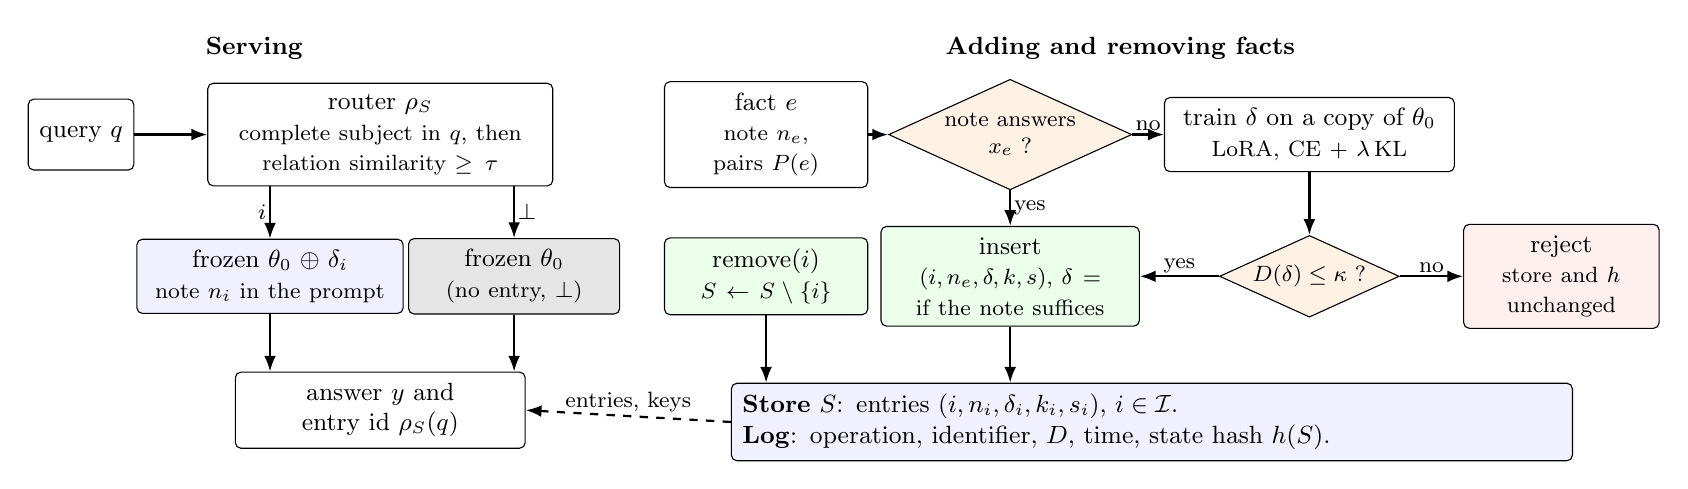
\begin{tikzpicture}[
  font=\small,
  box/.style={draw, rounded corners=2pt, align=center, inner sep=4pt, minimum height=9mm},
  base/.style={box, fill=black!10},
  store/.style={box, fill=blue!6},
  gate/.style={draw, diamond, aspect=2.2, align=center, inner sep=1pt, fill=orange!10, font=\footnotesize},
  arr/.style={-{Latex[length=2mm]}, thick},
  darr/.style={-{Latex[length=2mm]}, thick, dashed},
  lbl/.style={font=\footnotesize, inner sep=1pt},
  title/.style={font=\bfseries\small},
]
% ---------------- serve path
\node[title] (st) at (0,3.2) {Serving};
\node[box] (q) at (-2.2,2.1) {query $q$};
\node[box, text width=4.1cm] (r) at (1.6,2.1)
  {router $\rho_S$\\{\footnotesize complete subject in $q$, then relation similarity $\ge\tau$}};
\node[store, text width=3.1cm] (ex) at (0.2,0.3) {frozen $\theta_0\oplus\delta_i$\\{\footnotesize note $n_i$ in the prompt}};
\node[base, text width=2.4cm] (bs) at (3.3,0.3) {frozen $\theta_0$\\{\footnotesize (no entry, $\bot$)}};
\node[box, text width=3.4cm] (y) at (1.6,-1.4) {answer $y$ and entry id $\rho_S(q)$};
\draw[arr] (q) -- (r);
\draw[arr] ([xshift=-14mm]r.south) -- node[lbl, left]{$i$} ([xshift=-14mm]r.south |- ex.north);
\draw[arr] ([xshift=17mm]r.south) -- node[lbl, right]{$\bot$} ([xshift=17mm]r.south |- bs.north);
\draw[arr] (ex.south) -- (y.north -| ex.south);
\draw[arr] (bs.south) -- (y.north -| bs.south);

% ---------------- write path
\node[title] (wt) at (11.0,3.2) {Adding and removing facts};
\node[box, text width=2.3cm] (f) at (6.5,2.1) {fact $e$\\{\footnotesize note $n_e$, pairs $P(e)$}};
\node[gate] (ng) at (9.6,2.1) {note answers\\$x_e$ ?};
\node[box, text width=3.4cm] (tr) at (13.4,2.1)
  {train $\delta$ on a copy of $\theta_0$\\{\footnotesize LoRA, CE $+\ \lambda\,$KL}};
\node[gate] (g) at (13.4,0.3) {$D(\delta)\le\kappa$ ?};
\node[box, text width=2.2cm, fill=red!6] (rej) at (16.6,0.3) {reject\\{\footnotesize store and $h$ unchanged}};
\node[box, text width=3.0cm, fill=green!8] (com) at (9.6,0.3) {insert\\{\footnotesize $(i,n_e,\delta,k,s)$, $\delta=\varnothing$ if the note suffices}};
\node[box, text width=2.3cm, fill=green!8] (rev) at (6.5,0.3) {remove$(i)$\\{\footnotesize $S\leftarrow S\setminus\{i\}$}};
\draw[arr] (f) -- (ng);
\draw[arr] (ng) -- node[lbl, above]{no} (tr);
\draw[arr] (ng) -- node[lbl, right]{yes} (com);
\draw[arr] (tr) -- (g);
\draw[arr] (g) -- node[lbl, above]{no} (rej);
\draw[arr] (g) -- node[lbl, above]{yes} (com);

% ---------------- ledger / store
\node[store, text width=10.4cm, align=left] (led) at (11.4,-1.55)
  {\textbf{Store $S$}: entries $(i,n_i,\delta_i,k_i,s_i)$, $i\in\mathcal{I}$.\\ \textbf{Log}: operation, identifier, $D$, time, state hash $h(S)$.};
\draw[arr] (com.south) -- (com.south |- led.north);
\draw[arr] (rev.south) -- (rev.south |- led.north);
\draw[darr] (led.west) -- node[lbl, above]{entries, keys} (y.east);
\end{tikzpicture}}
\caption{Overview of Cerata. Left: the router selects at most one entry for a query; its
adapter, if any, is applied to the frozen base model and its note is placed in the
prompt. If no entry is selected, the base model answers. The answer is returned with the
identifier of the entry. Right: a fact whose note answers its edit prompt is stored as a
note only; otherwise a candidate adapter is trained on a separate copy of the base model
and inserted only if its divergence $D$ on held-out canary prompts is at most $\kappa$.
Removal deletes the entry. Bottom: the store and the log.}
\label{fig:arch}
\end{figure*}


Fig.~\ref{fig:arch} gives an overview of the system, and Algorithm~\ref{alg:txn} lists
its operations. This section describes the revised system; Section~\ref{sec:v3}
describes the first version and how it differed.

\subsection{Entries: Notes and Adapters}

Every fact is stored with a note, the statement $n_e$, which is served in the system
prompt together with the instruction ``Use the context even if it contradicts what you
know.'' A note is free to store and is removed exactly by deleting it. A note is not
always sufficient, because the base model may prefer its own answer. If the note does
not produce the target for the edit prompt at write time, the fact also receives an
adapter (the tiered store, Section~\ref{sec:tiered}). An entry with both is served with
the adapter active and the note in the prompt, which we found to be the most accurate
serving mode and use as the default.

\subsection{Adapters}

An adapter is a rank-16 LoRA update~\cite{hu2022lora} of the query and value projections
in every layer, trained from a fresh copy of the base model on two pairs, a statement of
the fact and the edit prompt with its answer (Table~\ref{tab:hparams}). The loss is
\begin{multline}
\mathcal{L}(\delta)=\sum_{(u,v)\in P(e)}\mathrm{CE}\big(v\mid u;\theta_0\oplus\delta\big)\\
+\frac{\lambda}{|Q|}\sum_{c\in Q}\mathrm{KL}\big(p_{\theta_0}(\cdot\mid c)\,\big\|\,
p_{\theta_0\oplus\delta}(\cdot\mid c)\big),
\label{eq:loss}
\end{multline}
where $Q$ is a set of anchor prompts and the KL term is computed on the next-token
distribution. In the confirmatory stores, $Q$ consists of two generic prompts. In
Section~\ref{sec:leak} we test adding three prompts about the fact's own subject with
other relations, so that the adapter learns to leave other questions about its subject
unchanged.

\subsection{Divergence Check}
\label{sec:checkmethod}

Let $p_c=p_{\theta_0}(\cdot\mid c)$ and $\tilde p_c=p_{\theta_0\oplus\delta}(\cdot\mid c)$.
A candidate adapter is scored by the mean symmetric KL divergence
\begin{equation}
D(\delta)=\frac{1}{|C|}\sum_{c\in C}\big[\mathrm{KL}(p_c\,\|\,\tilde p_c)
+\mathrm{KL}(\tilde p_c\,\|\,p_c)\big]
\end{equation}
on a set $C$ of canary prompts and is inserted only if $D(\delta)\le\kappa$. The canary
set must be disjoint from the anchor prompts $Q$, since an adapter is trained to leave
$Q$ unchanged. We use 40 held-out prompts covering factual questions, arithmetic,
instructions and four other languages, and set $\kappa$ to the 99th percentile of $D$
over stored adapters (Section~\ref{sec:check}).

\subsection{Router}
\label{sec:router}

The router has no parameters that are trained on the stored facts and works in three
steps.
\begin{enumerate}
\item \emph{Entity match.} The query and the stored subjects are normalized (lower case,
hyphens and underscores replaced by spaces). A subject matches if it occurs in the query
on word boundaries, or if every token of the subject matches a consecutive query token,
exactly for tokens shorter than four characters and within an optimal string alignment
distance of 1 (2 for six or more characters) otherwise. All entries whose subject is the
longest matching subject are candidates. If there is none, the router returns $\bot$.
\item \emph{Clause.} Only the sentence of the query that contains the matched subject is
kept.
\item \emph{Relation key.} The subject is replaced by a placeholder, both in this clause
and in the fact's edit prompt, and a frozen sentence encoder embeds the two relation
texts. The candidate with the highest cosine similarity is selected if the similarity is
at least $\tau$. Router v4 uses a multilingual MiniLM
encoder~\cite{reimers2019sbert,reimers2020multilingual}; the default configuration uses
a relation encoder trained offline (Section~\ref{sec:leak}).
\end{enumerate}
The threshold is calibrated on a development split that is disjoint from the test facts:
500 CounterFact and 500 zsRE facts with other subjects, with their held-out paraphrases
as positives and questions about the same subjects with templates of other CounterFact
relations as negatives. We set $\tau$ to maximize Youden's $J$ on this split, which gives
$\tau=0.631$ ($J=0.725$). Youden's $J$ weighs a missed paraphrase and a wrong route
equally, but a wrong route is more costly: it changes answers that the base model would
have given (Section~\ref{sec:check}) and often inserts the stored answer
(Section~\ref{sec:locres}). We therefore also use a locality-oriented threshold, the
lowest $\tau$ that routes at most 5\% of the CounterFact negatives of the development
split. This gives $\tau=\sTheta$ for router v4 and $\tau=\xTheta$ for the trained
relation encoder of the default configuration (Section~\ref{sec:leak}).

\subsection{Removal, Update and Logging}

\revoke$(i)$ deletes entry $i$. Because a fact can be stored more than once in different
phrasings, removal by content deletes every entry with the same subject and answer. An
update is a removal followed by an addition. For serving, the selected adapter is written
into a LoRA slot of the model and all other slots are set to zero. The log records the
identifier, the outcome of the check, $D$, the training time and the state hash.
Attribution is checked by leaving one adapter out: an answer is attributed to fact $i$ if
the target appears when $\delta_i$ is active and not when it is suspended.

The system is implemented in Python on Hugging Face Transformers and PEFT, and adapters
are stored in fp32. In the version evaluated here, the log consists of the records kept
by the experiment scripts, and the leave-one-out check is a separate script. We have not
built a persistent audit service.

\begin{algorithm}[t]
\caption{Operations on the store}
\label{alg:txn}
\begin{algorithmic}[1]
\Function{Add}{$e$, $i$}
  \State $k\gets E(\text{relation text of } x_e)$
  \If{$f_{\theta_0}(x_e\mid n_e)$ contains $a_e$} \State $\delta\gets\varnothing$
  \Else
    \State $\delta\gets\arg\min\mathcal{L}$ on a fresh copy of $\theta_0$ \Comment{Eq.~\eqref{eq:loss}}
    \If{$D(\delta)>\kappa$} \State log$(\textsc{reject},i)$ and \Return \EndIf
  \EndIf
  \State $S\gets S\cup\{(i,n_e,\delta,k,s_e)\}$; log$(\textsc{add},i,h(S))$
\EndFunction
\Function{Serve}{$q$}
  \State $j\gets\rho_S(q)$
  \State \Return $\big(f_{\theta_0\oplus\delta_j}(q\mid n_j),\ j\big)$ \Comment{$j=\bot$: base}
\EndFunction
\Function{Remove}{$i$}
  \State $S\gets S\setminus\{i\}$; log$(\textsc{remove},i,h(S))$
\EndFunction
\end{algorithmic}
\end{algorithm}

% ===========================================================================
\section{Exploratory Study}
\label{sec:lessons}

The adapter design was developed in a sequence of small experiments, each registered
before it was run. Table~\ref{tab:lessons} summarizes the measurements that determined
each design choice, and this section describes three of them.

% Exploratory measurements behind each design choice (slice record).
\begin{table}[t]
\centering
\caption{Exploratory measurements that determined the design
(Qwen2.5-1.5B-Instruct, 18 facts unless stated otherwise).}
\label{tab:lessons}
\scriptsize
\setlength{\tabcolsep}{3pt}
\begin{tabular}{>{\raggedright\arraybackslash}p{1.9cm}>{\raggedright\arraybackslash}p{3.9cm}>{\raggedright\arraybackslash}p{1.8cm}}
\toprule
Design question & Measurement & Choice \\
\midrule
Combine adapters by summation & Summed: 0/18 facts; routed: 18/18. With 50 facts: summed 0.00 (synthetic), 0.00 (CF), 0.02 (zsRE); one sequentially trained adapter 0.08, 0.34, 0.80 & One adapter per query \\
\addlinespace
Capacity of one adapter & Jointly trained: 64 synthetic facts, 1.00; 256 CF facts, 1.00 & Grouping possible \\
\addlinespace
Training strength & lr $10^{-4}$, 8 steps: attribution 0.06, KL 0.18. lr $3{\cdot}10^{-4}$, 16 steps: attribution 1.00, KL 10.96 (max 22.1). With KL term: attribution 0.94, KL 0.93 & KL term, $\lambda=1$ \\
\addlinespace
Routing key & Held-out paraphrases routed: TF-IDF 1/6, base-model hidden state 3/6, MiniLM 5/6 (6/6 with one paraphrase in training) & Sentence encoder \\
\addlinespace
Distractor rejection & Same question with unseen subject (50 synthetic facts): embeddings only 0.00; with entity filter 1.00 & Entity filter \\
\addlinespace
Routing after updates & Removing and adding a fact changed 0 other routing decisions & Fixed keys \\
\addlinespace
Failed additions & Over-threshold candidate ($D=21.6$), training exception, empty input: store and hash unchanged & Check before insert \\
\bottomrule
\end{tabular}
\end{table}


\subsection{Summing Adapters}
The simplest store would keep the sum of all adapters in a single LoRA module, so that
removal would be a subtraction. This did not work. With three facts on the 1.5B model,
adding the second adapter erased the first fact, and adding the third erased all three.
With 18 facts the sum answered none of them, and with 50 CounterFact or zsRE facts it
answered 0\% and 2\%. The same adapters, applied one at a time by a router, answered all
18. A single adapter trained sequentially on all facts answered 8\% of synthetic facts
and 34\% of CounterFact facts (80\% on zsRE, where the base model already knows many
answers). The problem is not the capacity of a rank-16 update, since one adapter trained
jointly on 256 CounterFact facts answers all of them (Section~\ref{sec:capacity}). We
attribute the failure to interference between independently trained
updates~\cite{ilharco2023taskarithmetic,yadav2023ties} and therefore apply one adapter
per query.

\subsection{Training Strength and the KL Penalty}
With 18 routed adapters, a weak setting (learning rate $10^{-4}$, 8 steps) changed the
anchor distributions little (mean symmetric KL 0.18) but did not learn the facts
(leave-one-out attribution 6\%). The setting that learned every fact ($3\cdot10^{-4}$,
16 steps) produced a mean divergence of 10.96 and a maximum of 22.1. Adding the KL term
of Eq.~\eqref{eq:loss} with $\lambda=1$ kept the facts and reduced the mean divergence to
0.93.

\subsection{Routing Keys}
On held-out paraphrases of six facts, TF-IDF character n-grams routed one correctly, and
the last-token hidden state of the base model routed three, because all short queries
had similarities above 0.9 to all keys. A multilingual MiniLM sentence encoder separated
the keys and routed five of six. In a 50-fact pilot, however, every distractor that asked
the same question about an unseen subject was routed to an adapter, since the question
template dominates the sentence embedding. Requiring a known subject before comparing
embeddings raised abstention from 0\% to 100\%. This entity filter is the origin of the
first version's router.

% ===========================================================================
\section{Experimental Setup}
\label{sec:setup}

\subsection{Model and Data}
The base model is Qwen2.5-1.5B-Instruct~\cite{qwen2024qwen25}, used in bf16 with its
chat template on a single 8\,GB GPU. Facts are drawn from the ROME versions of
CounterFact~\cite{meng2022rome} and zsRE~\cite{levy2017zeroshot,decao2021editing}.
CounterFact provides counterfactual targets that the base model does not produce. For
zsRE we use the reference answer, which the base model often knows already. We keep items
whose target is a single token and whose paraphrase contains the subject, shuffle the
remaining items with seed $N$ and take the first $N=1000$. Each fact has an edit prompt,
a held-out paraphrase (the first paraphrase prompt in CounterFact and the rephrased
question in zsRE) and a distractor, the edit prompt with the subject replaced by one of
five synthetic names. A set of synthetic facts with five relations is used for pilots
and router tests.

\subsection{Locality Queries}
Besides the synthetic distractors, we test three kinds of queries that should not use a
stored fact. On CounterFact, the dataset's neighborhood prompts ask the same relation
about a different real subject, and other-relation prompts ask about a stored subject
with the template of a randomly drawn other CounterFact relation, for example
``Vishwaroopam plays as'' for the stored fact about the original language of
Vishwaroopam. On zsRE we use the dataset's locality questions, which are drawn from
Natural Questions.

\subsection{Metrics}
An answer is correct if the lower-cased target occurs in the lower-cased greedy output.
Efficacy is measured on the edit prompts, which are part of each adapter's training data
and define the routing keys; it measures whether a fact was stored and can be retrieved.
The held-out paraphrases are the test of generalization. Route accuracy is the fraction of
edit prompts routed to their own fact. A query shows leakage if its output contains a
stored answer that the base model's output for the same query does not contain. For
removal, we remove the first 100 facts and measure the fraction of their edit prompts
whose correctness equals that of the base model before training (return) and the
accuracy on the 900 remaining facts (retention). Confidence intervals are 95\% percentile
bootstrap intervals over facts with 2000 resamples~\cite{efron1994bootstrap}; differences
between arms are paired.

\subsection{Baselines}
The note arm is our retrieval baseline. It uses the same router and serves the selected
fact's statement in the instructed system prompt; plain, question-answer and few-shot
formats performed worse in pilots. GRACE and WISE are the EasyEdit
implementations~\cite{wang2024easyedit} with their Qwen2.5 settings adapted to 28 layers
(GRACE at layer 18 with 50 iterations, WISE at layer 23 with 70 iterations in retrieval
mode), run in fp16 as 200 sequential edits on CounterFact, with and without a WISE merge
after edit 200. Both are scored with our protocol under the chat template and on the
plain edit prompt for which they were designed.

\subsection{Pre-Registration}
Arms, metrics, thresholds and predictions were committed before each run. This includes
the revised router, the calibration rules, the held-out canary set, the tiered policy and
the leakage experiments of Section~\ref{sec:leak}, which were registered after the
results that motivated them and before their own evaluation, together with a rule for
selecting the default configuration. Where a prediction failed, we say so.

% ===========================================================================
\section{The First Version and Its Failures}
\label{sec:v3}

% T3 - confirmatory readings at N=1000 (prereg SS56/58/59/62/64). Routed rows are the
% SS64 end-to-end re-evaluation; macros are generated into numbers.tex.
\begin{table}[t]
\centering
\caption{The first version (router v3) at $N=1000$ (Qwen2.5-1.5B-Instruct) with 95\%
bootstrap intervals. Unless noted, every query is served with the adapter selected by the
router, or by the base model if the router returns $\bot$.}
\label{tab:guarantees}
\footnotesize
\setlength{\tabcolsep}{3pt}
\resizebox{\columnwidth}{!}{%
\begin{tabular}{lcc}
\toprule
 & CounterFact & zsRE \\
\midrule
\multicolumn{3}{l}{\emph{Serving}} \\
Efficacy & $\cfEff\,[\cfEffCI]$ & $\zsEff\,[\zsEffCI]$ \\
Paraphrase accuracy & $\cfPara\,[\cfParaCI]$ & $\zsPara\,[\zsParaCI]$ \\
Route accuracy & $\cfRoute$ & $\zsRoute^{\dagger}$ \\
Paraphrase route accuracy & $\cfParaRoute$ & $\zsParaRoute$ \\
Abstention on distractors ($\ge 0.95$) & $\cfAbst$ & $\zsAbst$ \\
No leakage on distractors & $\cfNoLeak\,[\cfNoLeakCI]$ & $\zsNoLeak\,[\zsNoLeakCI]$ \\
\addlinespace
Efficacy, own adapter served & $0.999\,[.997,1]$ & $0.996\,[.992,.999]$ \\
\midrule
\multicolumn{3}{l}{\emph{Removal of the first 100 facts}} \\
Gone & $\cfGone\,[\cfGoneCI]$ & $\zsGone^{*}\,[\zsGoneCI]$ \\
Return to base answer & $\cfReturn\,[\cfReturnCI]$ & $\zsReturn\,[\zsReturnCI]$ \\
Retention, 900 facts ($\ge 0.98$) & $\cfRetain\,[\cfRetainCI]$ & $\zsRetain\,[\zsRetainCI]$ \\
Removal time & $\cfRevMs$\,ms & $\zsRevMs$\,ms \\
\midrule
\multicolumn{3}{l}{\emph{Divergence and attribution}} \\
Divergence $D$, mean / p95 / max & $.022\,/\,.052\,/\,.092$ & $.018\,/\,.043\,/\,.087$ \\
Rejected additions ($\kappa=2$) & $0/1000$ & $0/1000$ \\
Leave-one-out attribution ($\ge 0.95$) & $1.00$ ($100/100$) & not measured \\
\midrule
\multicolumn{3}{l}{\emph{Cost}} \\
Storage per fact (fp32) & $8.7$\,MB & $8.7$\,MB \\
Training time per fact & $8.5$\,s & $12.4$\,s \\
\bottomrule
\end{tabular}}
\\[2pt]
{\scriptsize $^{\dagger}$All 210 routing errors select a fact with the same subject
and answer; 208 are answered correctly. $^{*}$The base model answers 44 of these 100
prompts correctly before training. On CounterFact it answers none, so gone and return
coincide.}
\end{table}


The first version differed from the system of Section~\ref{sec:method} in three ways.
Its router compared the sentence embedding of the whole query with that of the whole edit
prompt, and its entity filter accepted a candidate if a single token of four or more
characters matched approximately. Facts were served by adapters only. The divergence
check used the two anchor prompts of the KL term with $\kappa=2.0$.
Table~\ref{tab:guarantees} reports its results at $N=1000$.

\subsection{What Held}
The first version answered \cfEffPct\% and \zsEffPct\% of the edit prompts, the outputs
for \cfNoLeakPct\% and \zsNoLeakPct\% of synthetic distractors contained no stored answer,
\cfRetainPct\% and \zsRetainPct\% of the facts were retained after 100 removals, and
leave-one-out attribution was 100\% for 100 CounterFact facts with an unchanged state
hash. On CounterFact, \cfReturnPct\% of the removed facts returned to the base model's
answer. A retrieval baseline instructed to follow its context answered 83.7\% of the
CounterFact edit prompts (Fig.~\ref{fig:scaling}).

% F2 - CounterFact efficacy vs N: the parametric store vs retrieval (prereg SS16/19/31/34/37/64).
\begin{figure}[t]
\centering
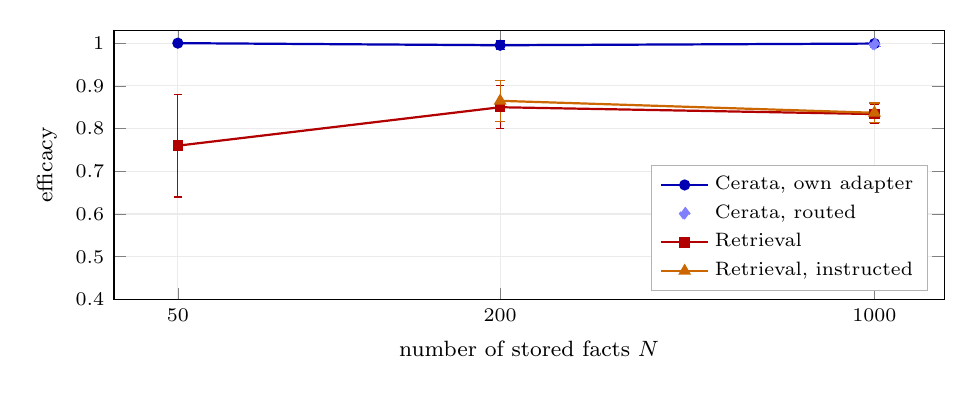
\begin{tikzpicture}
\begin{axis}[
  width=\columnwidth, height=5.0cm,
  xmode=log, log basis x=10,
  xtick={50,200,1000}, xticklabels={50,200,1000},
  xmin=38, xmax=1350,
  ymin=0.4, ymax=1.03,
  ytick={0.4,0.5,0.6,0.7,0.8,0.9,1.0},
  xlabel={number of stored facts $N$},
  ylabel={efficacy},
  legend style={font=\scriptsize, at={(0.98,0.03)}, anchor=south east, draw=black!30},
  legend cell align=left,
  grid=major, grid style={black!8},
  tick label style={font=\scriptsize}, label style={font=\footnotesize},
  error bars/y dir=both, error bars/y explicit,
]
\addplot[thick, blue!70!black, mark=*, mark size=1.6pt]
  coordinates {(50,1.00)+-(0,0) (200,0.995)+-(0,0.01) (1000,0.999)+-(0,0.002)};
\addlegendentry{Cerata, own adapter}
\addplot[thick, blue!50, dashed, mark=diamond*, mark size=2.2pt, only marks]
  coordinates {(1000,\cfEff)+-(0,\cfEffErr)};
\addlegendentry{Cerata, routed}
\addplot[thick, red!70!black, mark=square*, mark size=1.5pt]
  coordinates {(50,0.76)+-(0,0.12) (200,0.85)+-(0,0.05) (1000,0.834)+-(0,0.023)};
\addlegendentry{Retrieval}
\addplot[thick, orange!80!black, mark=triangle*, mark size=1.9pt]
  coordinates {(200,0.865)+-(0,0.048) (1000,0.837)+-(0,0.023)};
\addlegendentry{Retrieval, instructed}
\end{axis}
\end{tikzpicture}
\caption{Efficacy on CounterFact for different numbers of stored facts, with 95\%
bootstrap intervals. Retrieval and Cerata use the same router. ``Own adapter'' serves
each edit prompt with its own adapter; ``routed'' uses the router's selection
(Section~\ref{sec:v3}).}
\label{fig:scaling}
\end{figure}


\subsection{What Failed}
Three results contradicted the claims we had made for this version.

\emph{Paraphrases.} CounterFact paraphrase accuracy was \cfParaPct\%. The adapters
themselves generalize: served directly, they answered 86\% to 90\% of the paraphrases.
The router sent only 36\% of paraphrases to an adapter, and all 636 others passed the
entity filter and fell below the similarity threshold (median similarity 0.53 against
$\tau=0.656$). CounterFact paraphrase prompts begin with an unrelated sentence, for
example ``In 1978 her father suffered a heart attack and died. The original language of
Vishwaroopam was,'' which pulls the embedding of the whole query away from the key. On
the 362 paraphrases that did reach the correct adapter, the adapter answered 86.5\% and
instructed retrieval 81.8\%, a paired difference of 4.7 percentage points (95\% CI $-0.3$
to 9.7). The advantage over retrieval was therefore established only on the prompts the
adapters were trained on.

\emph{Locality.} The synthetic distractors were the easiest case. Other questions about
a stored subject passed the entity filter by construction and exceeded the threshold in
78.2\% of cases, and 34.6\% of their outputs contained the stored answer
(Table~\ref{tab:locality}). Neighborhood prompts were routed in 9.8\% of cases, all
through a single shared token such as ``Jean'' in ``Jean-Baptiste Say'' and ``Jean
Galland.'' Every query that was not routed received exactly the base model's output, and
nearly every routed one did not, so locality equaled the router's abstention rate.

\emph{Divergence check.} No adapter came close to $\kappa=2.0$ (maximum 0.092 over 2000
additions), because the check used the two prompts the KL term trains on. Section~\ref{sec:check}
shows that this measure understates the effect of an adapter seventeen-fold.

\subsection{Diagnosis}
The first two failures have one cause. Comparing whole queries mixes the subject, which
the entity filter already handles, with the relation, which the similarity should judge.
A leading sentence lowers the similarity of a correct paraphrase, while a question about
another relation of the same subject keeps a high similarity because the subject tokens
dominate the shared part. Matching single tokens lets unrelated subjects with a common
first name enter the candidate set. The revised router of Section~\ref{sec:router}
addresses these points directly: it requires the complete subject, restricts the query
to the clause that contains it, removes the subject from both texts before comparing,
and calibrates $\tau$ on negatives of the kind that failed.

We also found an error in our evaluation script while preparing this analysis. It served
an edit prompt with its own adapter whenever the router selected any adapter. All numbers
in this paper come from a re-evaluation of the saved adapters that uses the router's
actual selection; the error had changed efficacy by at most 0.2 percentage points.

% Locality on CounterFact by query type, router v3 vs v4 (prereg SS64/65/67).
\begin{table}[t]
\centering
\caption{Locality on CounterFact ($N=1000$) for three types of queries that should not
use a stored fact, with the first router (v3) and router v4. ``Routed'' is the fraction
sent to an adapter; ``leak'' the fraction of outputs that contain a stored answer the
base model's output does not contain. With v4, every query that is not routed receives
exactly the base model's output.}
\label{tab:locality}
\footnotesize
\setlength{\tabcolsep}{3pt}
\resizebox{\columnwidth}{!}{%
\begin{tabular}{lcccc}
\toprule
 & \multicolumn{2}{c}{v3} & \multicolumn{2}{c}{v4} \\
\cmidrule(lr){2-3}\cmidrule(lr){4-5}
Query type & Routed & Leak & Routed & Leak \\
\midrule
Synthetic subject, same question & $0.008$ & $0.008$ & $0.000$ & $0.000$ \\
Other subject, same relation & $0.098$ & $0.030$ & $\vCfEtwoRouted$ & $\vCfEtwoLeak$ \\
Stored subject, other relation & $0.782$ & $0.346$ & $\vCfEthreeRouted$ & $\vCfEthreeLeak$ \\
\bottomrule
\end{tabular}}
\end{table}


% ===========================================================================
\section{Results of the Revised System}
\label{sec:results}

All results in this section use the adapters stored for the first version, so that
differences are due to the router and the serving mode. Unless stated otherwise, they use
the Youden threshold $\tau=0.631$; Section~\ref{sec:leak} compares it with the
locality-oriented threshold.

% Routing with the first router (v3) and router v4 on the N=1000 test facts (prereg SS66).
\begin{table}[t]
\centering
\caption{Routing on the test facts with the first router (v3) and router v4. ``Routed''
is the fraction of queries sent to any adapter; ``correct'' the fraction sent to the
fact's own adapter. Router v4's threshold was calibrated on a disjoint dev split.}
\label{tab:router}
\footnotesize
\setlength{\tabcolsep}{4pt}
\resizebox{\columnwidth}{!}{%
\begin{tabular}{llcc}
\toprule
Set & Query & v3 & v4 \\
\midrule
CounterFact & Edit prompt, correct & $0.997$ & $0.998$ \\
 & Paraphrase, correct & $0.362$ & $0.814$ \\
 & Synthetic subject, routed & $0.008$ & $0.000$ \\
 & Neighborhood prompt, routed & $0.098$ & $0.018$ \\
 & Stored subject, other relation, routed & $0.782$ & $0.290$ \\
\midrule
zsRE & Edit prompt, correct & $0.784$ & $1.000$ \\
 & Paraphrase, routed & $0.985$ & $0.964$ \\
 & Synthetic subject, routed & $0.033$ & $0.000$ \\
 & NQ question (\texttt{loc}), routed & $0.000$ & $0.000$ \\
\midrule
Siblings & Original fact selected & n/a & $0.998$ \\
 & Added sibling selected & n/a & $0.995$ \\
\midrule
Stress (50) & Transposed characters & $1.00$ & $1.00$ \\
 & Last character dropped & $1.00$ & $0.00$ \\
 & First token of subject only & $0.80$ & $0.00$ \\
\bottomrule
\end{tabular}}
\end{table}


\subsection{Routing}
Table~\ref{tab:router} compares the two routers on the test facts. Router v4 sends
\vCfParaRoutePct\% of CounterFact paraphrases to the correct adapter (36.2\% with v3),
routes 29.0\% of other-relation prompts (78.2\%) and 1.8\% of neighborhood prompts (9.8\%),
and routes no synthetic distractor and no zsRE locality question. On zsRE every edit
prompt reaches its own fact, compared with 78.4\% for v3, whose errors selected rephrased
copies of the same fact. To test conflicting facts, we added to the store a second fact
for every CounterFact subject with another relation; v4 selected the original fact for
99.8\% of the original edit prompts and the added fact for 99.5\% of its prompts. The
price of requiring the complete subject is recall on incomplete mentions: on 50
synthetic facts, subjects with a dropped final character or only their first token are
no longer routed.

% Revised system at N=1000: router v4 with three serving arms (prereg SS67/68).
\begin{table}[t]
\centering
\caption{The revised system at $N=1000$ with router v4. Each query is served with the
routed adapter, with the routed fact's note in an instructed prompt, or with both. The
difference is the paired difference between adapter and note in percentage points.}
\label{tab:serving}
\footnotesize
\setlength{\tabcolsep}{3pt}
\resizebox{\columnwidth}{!}{%
\begin{tabular}{llcc}
\toprule
 & & CounterFact & zsRE \\
\midrule
Edit prompt & adapter & $\vCfEff\,[\vCfEffCI]$ & $\vZsEff\,[\vZsEffCI]$ \\
 & note & $\vCfEffRet$ & $\vZsEffRet$ \\
 & both & $\vCfEffBoth$ & $\vZsEffBoth$ \\
\midrule
Paraphrase & adapter & $\vCfPara\,[\vCfParaCI]$ & $\vZsPara\,[\vZsParaCI]$ \\
 & note & $\vCfParaRet$ & $\vZsParaRet$ \\
 & both & $\vCfParaBoth\,[\vCfParaBothCI]$ & $\vZsParaBoth\,[\vZsParaBothCI]$ \\
 & adapter $-$ note (pp) & $\vCfParaDiff$ (\vCfParaDiffCI) & $\vZsParaDiff$ (\vZsParaDiffCI) \\
\midrule
Removal of 100 & return to base & $\vCfReturn$ & $\vZsReturn$ \\
 & return, removal by content & n/a & $\vZsReturnContent$ \\
 & retention of 900 & $\vCfRetain$ & $\vZsRetain$ \\
\midrule
Tiered store & facts needing an adapter & $\vCfTierFrac$ & $\vZsTierFrac$ \\
 & efficacy / paraphrase & $\vCfTierEff$ / $\vCfTierPara$ & $\vZsTierEff$ / $\vZsTierPara$ \\
\bottomrule
\end{tabular}}
\end{table}


\subsection{Serving}
Table~\ref{tab:serving} reports the three serving modes at $N=1000$. Efficacy on the edit
prompts is unchanged (\vCfEffPct\% and \vZsEffPct\% with the adapter). Paraphrase accuracy
on CounterFact rises from 32.3\% to \vCfParaPct\% with the adapter. The adapter now
outperforms the note on paraphrases by \vCfParaDiff\ percentage points on CounterFact
(95\% CI \vCfParaDiffCI) and \vZsParaDiff\ on zsRE (\vZsParaDiffCI), so its advantage holds
beyond the trained prompts. Serving the adapter together with the note is the most
accurate mode: it answers \vCfParaBothPct\% of CounterFact paraphrases and \vZsParaBothPct\%
of zsRE paraphrases, and 97.9\% of the CounterFact paraphrases that reach the correct fact,
compared with 81.5\% for the adapter alone and 76.5\% for the note alone. The note supplies
the fact in the wording of the query's context, and the adapter overrides the base model's
prior; each covers cases the other misses.

\subsection{Locality}
\label{sec:locres}
With v4, none of the synthetic distractors and none of the 1000 zsRE locality questions
is routed, and all of them receive the base model's output. On CounterFact, neighborhood
prompts leak in \vCfEtwoLeakPct\% of cases (3.0\% with v3) and other-relation prompts in
\vCfEthreeLeakPct\% (34.6\%; Table~\ref{tab:locality}). The remaining leakage comes from
the 29\% of other-relation prompts that v4 still routes: when such a prompt is routed, the
adapter produces a stored answer in 64\% of cases, and 166 of these 186 outputs contain
the routed fact's own answer. The leakage is not specific to the adapter. Serving the note
instead leaks in \vCfEthreeLeakNotePct\% of the prompts and serving both in
\vCfEthreeLeakBothPct\%, because the instructed model also uses a note about one relation
of a subject to answer another question about that subject.

\subsection{Removal}
On CounterFact, removal now returns all 100 removed facts to the base model's answer; the
four exceptions of the first version were routes to a similar subject that v4 no longer
takes. On zsRE, where the base model already answers 44 of the 100 prompts, \vZsReturnPct\%
return. The remaining cases are rephrased copies of the removed facts that are still
stored. Removal by content, which also deletes the \vZsContentExtra\ entries with the same
subject and answer, returns all 100. Retention of the other facts is \vCfRetainPct\% and
\vZsRetainPct\%, and a removal takes about 2.5\,ms.

\subsection{Tiered Store}
\label{sec:tiered}

A note costs nothing to store, while an adapter occupies 8.7\,MB in fp32 and takes 8.5\,s
to train. With the policy of Algorithm~\ref{alg:txn}, which gives a fact an adapter only
if its note fails on the edit prompt at write time, \vCfTierFracPct\% of CounterFact facts
and \vZsTierFracPct\% of zsRE facts need an adapter, a five- to six-fold reduction in
adapter storage. The tiered store answers \vCfTierEffPct\% and \vZsTierEffPct\% of the edit
prompts and \vCfTierParaPct\% and \vZsTierParaPct\% of the paraphrases, close to the
adapter-only store (\vCfParaPct\% and \vZsParaPct\%). Storing an adapter for every fact
and serving both gives the highest paraphrase accuracy (\vCfParaBothPct\% on CounterFact)
at the full storage cost. The choice is a trade-off between storage and paraphrase
accuracy that a deployment can make per fact. At the locality-oriented threshold, the
tiered store answers \sCfParaTierPct\% of the CounterFact paraphrases and leaks into
\sCfEthreeLeakTieredPct\% of the other-relation prompts.

\subsection{Divergence Check}
\label{sec:check}

% Divergence check: in-sample vs held-out canaries, harmful candidates, wrong routes (SS69).
\begin{table}[t]
\centering
\caption{Divergence $D$ on the two canary prompts used in training and on 40 held-out
canary prompts, for 100 stored adapters and for 10 harmful candidates trained without
the KL term. The last row is the fraction of 200 questions the base model answers
correctly that remain correct when a randomly chosen adapter is applied.}
\label{tab:check}
\footnotesize
\setlength{\tabcolsep}{4pt}
\resizebox{\columnwidth}{!}{%
\begin{tabular}{lcc}
\toprule
 & Training canaries & Held-out canaries \\
\midrule
Stored adapters, mean / max & $0.022$ / $0.078$ & $0.364$ / $1.07$ \\
Harmful candidates, min / max & $2.03$ / $32.9$ & $3.46$ / $28.8$ \\
Threshold $\kappa$ & $2.0$ (fixed) & $0.97$ (p99 of stored) \\
Harmful candidates rejected & 10/10 & 10/10 \\
\midrule
Correct answers kept under a wrong route & \multicolumn{2}{c}{$0.72$} \\
\bottomrule
\end{tabular}}
\end{table}


For 100 stored adapters, the mean divergence on the two anchor prompts is \chkInMean,
and on the 40 held-out canary prompts \chkHeldMean, with a maximum of \chkHeldMax\
(Table~\ref{tab:check}). The anchor prompts thus understate the effect of an adapter
about seventeen-fold, because the KL term trains on them. To test whether the check can
reject a harmful adapter, we trained 10 candidates without the KL term at a learning rate
of $10^{-3}$ for 32 steps. Their held-out divergence is 3.46 to 28.8. With
$\kappa=\chkKappa$, the 99th percentile over the stored adapters, all 10 are rejected and
the closest harmful candidate lies 3.6 times above the threshold. The in-sample check
with $\kappa=2.0$ also rejects all 10, but the closest one scores 2.03, so it has no
margin. The cost of an incorrect route is substantial: when a randomly chosen adapter is
applied to 200 questions that the base model answers correctly, \chkWrongRoutePct\% of
the answers remain correct. Routing precision is therefore a safety property as well as
an accuracy property.

\subsection{Reducing Leakage}
\label{sec:leak}

% Attempts to reduce leakage into other questions about stored subjects (SS70-74).
\begin{table}[t]
\centering
\caption{Attempts to reduce leakage into other-relation prompts on CounterFact. Each row
reports paraphrase accuracy and leakage for the same serving arm; the first block uses
all 1000 facts, the last row the first 200, compared with their original adapters.}
\label{tab:leakage}
\footnotesize
\setlength{\tabcolsep}{3pt}
\resizebox{\columnwidth}{!}{%
\begin{tabular}{llcc}
\toprule
Change & Arm & Paraphrase & Leakage \\
\midrule
None (router v4, $\tau=0.631$) & adapter & $\vCfPara$ & $\vCfEthreeLeakAdapter$ \\
 & note & $\vCfParaRet$ & $0.140$ \\
 & both & $\vCfParaBoth$ & $\vCfEthreeLeakBoth$ \\
 & tiered & $\vCfTierPara$ & $\vCfEthreeLeakTiered$ \\
Store contrast & both & $0.764$ & $0.177$ \\
Base-model check & both & $0.798$ & $0.232$ \\
Threshold $\tau=\sTheta$ & adapter & $\sCfPara$ & $\sCfEthreeLeakAdapter$ \\
 & note & $\sCfParaRet$ & $\sCfEthreeLeakNote$ \\
 & both & $\sCfParaBoth$ & $\sCfEthreeLeakBoth$ \\
 & tiered & $\sCfParaTier$ & $\sCfEthreeLeakTiered$ \\
Generated keys, mpnet, & adapter & $\wCfPara$ & $\wCfEthreeLeakAdapter$ \\
\quad $\tau=\wTheta$ & note & $\wCfParaRet$ & $\wCfEthreeLeakNote$ \\
 & both & $\wCfParaBoth$ & $\wCfEthreeLeakBoth$ \\
 & tiered & $\wCfParaTier$ & $\wCfEthreeLeakTiered$ \\
Trained relation & adapter & $\xCfPara$ & $\xCfEthreeLeakAdapter$ \\
\quad encoder, $\tau=\xTheta$ & note & $\xCfParaRet$ & $\xCfEthreeLeakNote$ \\
 & both & $\xCfParaBoth$ & $\xCfEthreeLeakBoth$ \\
 & tiered & $\xCfParaTier$ & $\xCfEthreeLeakTiered$ \\
\midrule
Subject-local anchors (200) & adapter & $0.690\to0.550$ & $0.160\to0.090$ \\
 & both & $0.805\to0.805$ & $0.200\to0.185$ \\
\bottomrule
\end{tabular}}
\end{table}

% F3 - paraphrase accuracy vs leakage into other-relation prompts along the routing
% threshold (prereg SS74; data from make_numbers.py), with the alternatives of SS71-73.
\begin{figure}[t]
\centering
\begin{tikzpicture}
\begin{axis}[
  width=\columnwidth, height=5.6cm,
  xmin=0, xmax=0.25, ymin=0.3, ymax=0.95,
  xtick={0,0.05,0.10,0.15,0.20,0.25},
  xticklabels={0,.05,.10,.15,.20,.25},
  ytick={0.3,0.4,0.5,0.6,0.7,0.8,0.9},
  xlabel={leakage into other-relation prompts},
  ylabel={paraphrase accuracy},
  legend style={font=\scriptsize, at={(0.5,1.03)}, anchor=south, draw=black!30, legend columns=3},
  legend cell align=left,
  grid=major, grid style={black!8},
  tick label style={font=\scriptsize}, label style={font=\footnotesize},
]
\addplot[thick, blue!70!black, mark=*, mark size=1.1pt]
  table[x=leak_both, y=para_both] {figures/tradeoff.dat};
\addlegendentry{adapter and note}
\addplot[thick, orange!80!black, dashed, mark=square*, mark size=1.0pt]
  table[x=leak_adapter, y=para_adapter] {figures/tradeoff.dat};
\addlegendentry{adapter}
\addplot[only marks, red!70!black, mark=triangle*, mark size=2.6pt]
  coordinates {(0.177,0.764)};
\addlegendentry{store contrast}
\addplot[only marks, green!45!black, mark=diamond*, mark size=2.6pt]
  coordinates {(0.232,0.798)};
\addlegendentry{base-model check}
\addplot[only marks, violet!80!black, mark=pentagon*, mark size=2.6pt]
  coordinates {(\wCfEthreeLeakBoth,\wCfParaBoth) (\wCfEthreeLeakAdapter,\wCfPara)};
\addlegendentry{generated keys}
\addplot[only marks, black, mark=star, mark size=3.2pt, thick]
  coordinates {(\xCfEthreeLeakBoth,\xCfParaBoth) (\xCfEthreeLeakAdapter,\xCfPara)};
\addlegendentry{trained encoder}
\node[font=\scriptsize, anchor=north east] at (axis cs:0.237,0.795) {$\tau{=}0.631$};
\draw[black!50] (axis cs:0.063,0.589) -- (axis cs:0.094,0.475);
\node[font=\scriptsize, anchor=north west, inner sep=1pt] at (axis cs:0.092,0.475) {$\tau{=}0.757$};
\draw[black!60] (axis cs:0.063,0.589) circle (2.5pt);
\end{axis}
\end{tikzpicture}
\caption{CounterFact paraphrase accuracy against the fraction of other-relation prompts
whose output contains a stored answer, as the routing threshold $\tau$ increases from
0.631 (top right) to 0.963. Store contrast and the base-model check are the alternative
relevance tests of Section~\ref{sec:leak}, both served with adapter and note; each
lies on the curve that the threshold alone produces. Generated keys with all-mpnet-base-v2
at $\tau=\wTheta$ and the trained relation encoder at $\tau=\xTheta$ are shown for both
arms and lie above the curves.}
\label{fig:tradeoff}
\end{figure}


We tested eight changes that could reduce leakage into other-relation prompts
(Table~\ref{tab:leakage}), each registered with a prediction before it was run. The
first four did not improve on the trade-off that the routing threshold gives, the fifth
improved on it slightly, the sixth, a relation encoder trained for this comparison,
improved on it substantially for the relations it was trained on, and the last two,
training that encoder on a broader relation inventory and giving each fact negative keys,
added nothing.

\emph{Subject-local anchors.} We retrained the adapters of the first 200 CounterFact facts
with three additional anchor prompts in Eq.~\eqref{eq:loss}: questions about the fact's
own subject with the templates of three other CounterFact relations, excluding the
relation of the test prompts. With router v4, the retrained adapters reduce leakage on
these facts from 16.0\% to 9.0\% and the mean held-out divergence from 0.343 to 0.146.
They also learn the facts less well: efficacy falls from 100\% to 93.0\% and paraphrase
accuracy from 69.0\% to 55.0\%. Served together with the note, they answer as many
paraphrases as the original adapters (80.5\%), but the leakage of the note remains
(18.5\% against 20.0\%). With three anchor prompts and 32 training steps, an adapter does
not separate the relation it should change from the other relations of its subject.

\emph{Store contrast.} A relation that is stored for another subject can serve as a
contrast. We accepted a route only if the selected key's similarity to the query's
relation text is at most a margin $m$ below that of the most similar key in the whole
store, with $m=0.33$ calibrated on the development split. This reduced the routed
other-relation prompts from 29.0\% to 20.8\% and the leakage with adapter and note from
\vCfEthreeLeakBothPct\% to 17.7\%, while paraphrase accuracy fell from \vCfParaBothPct\%
to 76.4\%.

\emph{Base-model check.} We asked the frozen base model whether the selected fact's
statement answers the query and used the difference between the logits of ``Yes'' and
``No'' as a score. On the routed development queries, the medians are 4.1 for correct
paraphrases and $-1.4$ for other-relation prompts, but the distributions overlap, and
the threshold that maximizes Youden's $J$ removes almost no routes. A third score, the
base model's log probability of the stored answer after the query relative to that after
the edit prompt, was eliminated on the development split. Its area under the ROC curve
was \aucTypePool, compared with \aucJudgePool\ for the base-model check and \aucRelPool\
for the relation similarity that the router already uses.

\emph{Threshold.} Raising $\tau$ above the Youden point trades paraphrase accuracy for
leakage along the curve in Fig.~\ref{fig:tradeoff}. The store contrast and the base-model
check lie on this curve, so neither adds information beyond the similarity itself. At
$\tau=\sTheta$, \sCfEthreeRoutedPct\% of the other-relation test prompts are routed, and
\sCfEthreeLeakBothPct\% leak with adapter and note (\sCfEthreeLeakNotePct\% with the note
alone). Paraphrase accuracy falls to \sCfParaBothPct\% on CounterFact and
\sZsParaBothPct\% on zsRE, while edit prompts are unaffected (\sCfEffBothPct\%). Every
route taken at $\tau=\sTheta$ is also taken at $\tau=0.631$, so the fraction of removed
facts that return to the base model's answer can only increase. The selection rule that
we registered before these runs chooses, among the configurations with at most 10\%
leakage, the one with the highest paraphrase accuracy. It selects adapter and note at
$\tau=\sTheta$, which was the default until the trained relation encoder described below
replaced it.

Above $\tau\approx0.72$, almost every routed other-relation prompt leaks, because the
prompts that remain ask nearly the same question as the stored fact. For 1.3\% of the
other-relation prompts, CounterFact uses the same template for both relations, for
example ``X is located in'' for the continent and for the country of a place; these
prompts account for 11 of the 63 leaking outputs at $\tau=\sTheta$. Most of the others
are near synonyms, such as ``The location of X is'' and ``X is located in'' or
``produced by'' and ``a product developed by.'' A router that compares relation texts
cannot separate such pairs, and for some of them the stored answer also answers the other
question.

\emph{Relation scorer and generated keys.} Finally, we tried to move the curve itself.
We compared four frozen sentence encoders, the MiniLM model of router v4,
all-mpnet-base-v2~\cite{song2020mpnet}, bge-large-en-v1.5~\cite{xiao2024cpack} and
e5-large-v2~\cite{wang2022e5}, and a cross-encoder trained to detect duplicate questions,
each with and without generated keys. A generated key is one of three rewrites of the
edit prompt that the base model produces at write time and that keep the subject; a
candidate's score is its maximum over the original and the generated keys. On the
development split, at the threshold that routes 5\% of the CounterFact negatives,
generated keys raised the fraction of correctly routed paraphrases by three to four
points for every sentence encoder, the choice of encoder changed it by less, and the
cross-encoder was the weakest scorer. The selected configuration, all-mpnet-base-v2 with
generated keys at $\tau=\wTheta$, raised this fraction from 67.7\% to 71.6\%, short of
the five points we had predicted. On the test sets it answers \wCfParaBothPct\% of the
CounterFact paraphrases with adapter and note (95\% CI \wCfParaBothCIPct) and leaks into
\wCfEthreeLeakBothPct\% of the other-relation prompts, which is better on both measures
than MiniLM at $\tau=\sTheta$ (\sCfParaBothPct\% and \sCfEthreeLeakBothPct\%); on zsRE it
answers \wZsParaBothPct\% of the paraphrases. We had required 65\% paraphrase accuracy
for replacing MiniLM, so this configuration was not adopted, although it was the first
change that moved the trade-off curve.

% Trained relation encoder: CounterFact results split by seen and held-out relations (SS76).
\begin{table}[t]
\centering
\caption{The trained relation encoder on CounterFact, split by whether the relations
involved were used in its training, compared with router v4 at $\tau=\sTheta$. Paraphrase
rows give the fraction routed to the correct fact; leakage rows the fraction of
other-relation prompts whose output with adapter and note contains a stored answer.}
\label{tab:relsplit}
\footnotesize
\setlength{\tabcolsep}{3pt}
\begin{tabular}{lccc}
\toprule
Queries & $n$ & Router v4 & Trained \\
\midrule
Paraphrase, seen relation & \xParaSeenN & $\xParaSeenDefRoute$ & $\xParaSeenRoute$ \\
Paraphrase, held-out relation & \xParaHeldN & $\xParaHeldDefRoute$ & $\xParaHeldRoute$ \\
\midrule
Leakage, both relations seen & \xEthreeSeenN & $\xEthreeSeenDef$ & $\xEthreeSeenLeak$ \\
Leakage, stored relation held out & \xEthreeStoredHeldN & $\xEthreeStoredHeldDef$ & $\xEthreeStoredHeldLeak$ \\
Leakage, query relation held out & \xEthreeQueryHeldN & $\xEthreeQueryHeldDef$ & $\xEthreeQueryHeldLeak$ \\
Leakage, both held out & \xEthreeBothHeldN & $\xEthreeBothHeldDef$ & $\xEthreeBothHeldLeak$ \\
\bottomrule
\end{tabular}
\end{table}


\emph{Trained relation encoder.} The general-purpose encoders differ little, and none of
them was trained to decide whether two questions ask for the same relation. We therefore
trained all-mpnet-base-v2 once, offline, on triplets of subject-masked relation texts:
an edit prompt, one of its paraphrases, and a template of another relation, with a
multiple-negatives ranking loss~\cite{henderson2017efficient} (7500 triplets, one epoch,
45\,s). The triplets come from 3000 CounterFact and 1500 zsRE facts whose subjects occur
neither in the development split nor in the test stores, and 11 of the 34 CounterFact
relations were left out of training entirely. The encoder is then frozen. It belongs to
the router, not to the store: keys are fixed once computed, and Propositions 1 to 3 hold
unchanged. With the selection rule above, it routes \xDevTprPct\% of the development
paraphrases at $\tau=\xTheta$, against 71.6\% for the best frozen configuration. On the
test sets it answers \xCfParaBothPct\% of the CounterFact paraphrases with adapter and
note (95\% CI \xCfParaBothCIPct) and leaks into \xCfEthreeLeakBothPct\% of the
other-relation prompts, and it answers \xZsParaBothPct\% of the zsRE paraphrases. Edit
prompts, synthetic distractors and zsRE locality questions are unaffected, and removal
on CounterFact remains complete. Both predictions that we had registered for replacing
the default held, so this configuration is the default.

Table~\ref{tab:relsplit} shows where the gain comes from. On relations seen in training,
\xParaSeenRoutePct\% of the paraphrases are routed to their fact, and leakage falls from
\xEthreeSeenDefPct\% to \xEthreeSeenLeakPct\%. On held-out relations, paraphrase routing
still improves, from \xParaHeldDefRoutePct\% to \xParaHeldRoutePct\%, but leakage does
not fall. The encoder has largely learned the inventory of relation templates in
CounterFact. The result therefore applies to a deployment whose relations are known in
advance, such as a store that follows a fixed schema. For new relations, the encoder
transfers part of the recall and none of the locality.

\emph{A broader relation inventory.} To test whether training on more relations transfers
locality to new ones, we trained two further encoders on templates for the 1785
item-valued Wikidata properties, four per property, written by the base model. Encoder
A saw none of the 34 CounterFact relations; encoder B added these templates to the
training data of the encoder above, again without the 11 held-out relations, and was
selected and evaluated in the same way. Encoder A routes \aCfParaRoutePct\% of the
CounterFact paraphrases correctly at the 5\% threshold, against \mpCfParaRoutePct\% for
the untrained all-mpnet-base-v2, so training on other relations transfers in part. The
gain falls on the 23 relations that the first encoder was trained on
(\aParaSeenRoutePct\% against \mpParaSeenRoutePct\%), not on the 11 held-out ones
(\aParaHeldRoutePct\% against \mpParaHeldRoutePct\%). Encoder B behaves like the encoder
trained on CounterFact alone: on held-out relations it routes \uParaHeldRoutePct\% of the
paraphrases and leaks into \uHeldLeakPct\% of the prompts that involve them, as before
(\xHeldLeakPct\%). Three of our four predictions for B failed, and the default is
unchanged. The held-out relations are hard for a reason that more relations in training
do not remove. Of the 33 leaking outputs under B that involve a held-out relation, 20
come from pairs that differ in nuance: country of origin and location of formation,
original language and language of the work, native and other languages, manufacturer and
developer, and location and administrative location. Where two relations differ in this
way, the boundary between them has to be learned from examples of that pair.

\emph{Negative keys.} Such examples could come from the base model at write time. For
each fact, the base model wrote five questions about the same subject that ask for
different but related information, and the router accepted a route only if the query was
closer to the fact's keys than to these negative keys by a margin calibrated on the
development split. The calibration gave the same development TPR with and without the
negative keys, and on the test set the routed fraction of other-relation prompts that
involve a held-out relation stayed at 5.9\%. The generated questions mostly ask for
unrelated attributes, such as a founding year or notable people, and rarely for the
neighboring relation that a query actually confuses; some even restate the stored
question. Since the routes differed from the trained encoder's only through the threshold,
we did not run the end-to-end evaluation that we had registered.

\subsection{Comparison with Editing Methods}

% T4 - baselines on CounterFact, same base model (prereg SS31/37/54/63/64).
\begin{table*}[t]
\centering
\caption{Comparison on CounterFact with Qwen2.5-1.5B-Instruct. ``Chat'' uses the chat
template; ``plain'' uses the edit prompt without a template, the format for which GRACE
and WISE were designed. GRACE and WISE (EasyEdit) were run as 200 sequential edits,
the note and Cerata with 1000 facts. The note and the first three Cerata rows use router v4 with $\tau=0.631$; the default uses the trained relation encoder (adapter and note). No
leakage refers to the synthetic distractors.}
\label{tab:baselines}
\footnotesize
\resizebox{\textwidth}{!}{%
\begin{tabular}{llcccccc}
\toprule
Method & Storage & $N$ & Efficacy (chat) & Efficacy (plain) & Paraphrase & No leakage & Removal \\
\midrule
Note (instructed retrieval) & context & $1000$ & $\vCfEffRet\,[\vCfEffRetCI]$ & n/a & $\vCfParaRet$ & $1.00$ & per entry \\
GRACE~\cite{hartvigsen2023grace} & key-value codebook & $200$ & $0.025$ & $1.00$ & $0.02$ & $1.00$ & none \\
WISE~\cite{wang2024wise} & side memory & $200$ & $0.07$ & $0.04$ & $0.06$ & $0.64$ & none \\
WISE, merged at 200 & side memory & $200$ & $0.125\,[.08,.17]$ & $0.05$ & $0.105$ & $0.27\,[.21,.335]$ & none \\
\midrule
Cerata, adapter & adapter per fact & $1000$ & $\vCfEff\,[\vCfEffCI]$ & n/a & $\vCfPara$ & $\vCfNoLeak$ & per entry \\
Cerata, adapter and note & adapter per fact & $1000$ & $\vCfEffBoth\,[\vCfEffBothCI]$ & n/a & $\vCfParaBoth$ & $\vCfNoLeak$ & per entry \\
Cerata, tiered & adapter for 16.2\% & $1000$ & $\vCfTierEff\,[\vCfTierEffCI]$ & n/a & $\vCfTierPara$ & $\vCfNoLeak$ & per entry \\
Cerata, default (trained router) & adapter per fact & $1000$ & $\xCfEffBoth\,[\xCfEffBothCI]$ & n/a & $\xCfParaBoth$ & $1.00$ & per entry \\
\bottomrule
\end{tabular}}
\\[3pt]
{\scriptsize EasyEdit's own metrics: GRACE token accuracy is 0.0 because the target
token differs when preceded by a space; WISE per-edit accuracy is 1.00 without and 0.66
with merging.}
\end{table*}


Table~\ref{tab:baselines} compares the official editing implementations with Cerata.
GRACE answers all 200 edits on the plain edit prompt but only 2.5\% under the chat
template, because its keys are activations of the last token of the plain prompt and
the chat template changes this token. WISE reports a per-edit accuracy of 100\%, while
the model after all 200 edits answers 7\% of them. With a merge after edit 200, the final
accuracy rises to 12.5\%, the fraction of distractors without leakage falls from 64\% to
27\%, and the accuracy on plain prompts is 5\%, so the decline is not caused by the chat
template. These results agree with earlier findings that editing results depend on the
evaluation format and on whether accuracy is measured after each edit or after all
edits~\cite{yang2025mirage,gupta2024forgetting}. Neither implementation provides an
operation for removing a single edit. Because GRACE and WISE were run with 200 facts and
Cerata with 1000, the comparison is descriptive.

\subsection{Grouped Adapters}
\label{sec:capacity}

% T4 - grouped capacity (prereg SS50/61).
\begin{table}[t]
\centering
\caption{Grouped capacity: one delta carrying $k$ facts (seeded; base-referenced
leakage; base hit rate $0.0$).}
\label{tab:capacity}
\footnotesize
\begin{tabular}{lccc}
\toprule
$k$ & Efficacy & KLD & Leakage \\
\midrule
$64$ & $0.984$ & $0.002$ & $0.3$ \\
$128$ & $1.00$ & $0.002$ & $0.1$ \\
$256$ & $1.00$ & $0.007$ & $0.3$ \\
\bottomrule
\end{tabular}
\end{table}


One adapter of the same rank trained jointly on $k$ CounterFact facts answers 98.4\%,
100\% and 100\% of its facts at $k=64$, 128 and 256, with a divergence on the anchor
prompts of at most 0.007 (Table~\ref{tab:capacity}), and its paraphrase accuracy is 58\%,
70\% and 66\%. A grouped adapter also produces the answer for one to three of ten held-out
facts that the base model does not answer, and removing one of its facts requires
retraining the group. Grouping is therefore an alternative to the tiered store for
reducing storage, at the cost of coarser removal and some leakage.

% ===========================================================================
\section{Extensions}
\label{sec:loop}

This section reports smaller experiments with the first version on three questions that
arise during deployment: which facts should receive adapters, how updates behave across
sessions, and whether the approach applies to a vision-language model.
Table~\ref{tab:loop} summarizes the results. The experiments are exploratory and
involve few facts.

% Extensions (exploratory, slice record).
\begin{table}[t]
\centering
\caption{Extension experiments. Top: policies for storing facts as adapters on a stream
of 6 facts queried three times and 12 queried once, with retrieval as the default
memory. Bottom: the store on Qwen3-VL-2B.}
\label{tab:loop}
\scriptsize
\setlength{\tabcolsep}{4pt}
\resizebox{\columnwidth}{!}{%
\begin{tabular}{lcc}
\toprule
Policy & Adapters & Facts answered \\
\midrule
Store after two queries & 6 & 16/18 \\
$\epsilon$-greedy, decide before answering & 0 & 15/18 \\
UCB1, decide before answering & 17 & 17/18 \\
UCB1, decide after an incorrect answer & 3 & 18/18 \\
\midrule
Vision-language test & \multicolumn{2}{c}{Result} \\
\midrule
Two facts keyed by images (CLIP, $\tau=0.97$) & \multicolumn{2}{c}{2/2 answered; distractor images not routed} \\
Adapter that changes a canary answer & \multicolumn{2}{c}{$D=23.9$, rejected; hash unchanged} \\
Update, then removal & \multicolumn{2}{c}{new answer served; hash restored} \\
Save and reload & \multicolumn{2}{c}{same hash; 2/2 answered} \\
Adapter trained with negative images & \multicolumn{2}{c}{answers only for its scene and variants} \\
Controller with such adapters & \multicolumn{2}{c}{4 adapters; 4/4 answered; no leakage} \\
\bottomrule
\end{tabular}}
\end{table}


\subsection{Choosing Which Facts to Store as Adapters}
We combined adapters with a retrieval memory of notes and used a controller to decide
when a fact should receive an adapter. The stream contains 6 facts that are queried three
times and 12 that are queried once. A rule that gives an adapter to every fact queried at
least twice created 6 adapters and answered 16 of 18 facts; the two failures were facts
queried only once on which retrieval fails. Bandit controllers that decide before the
query is answered performed poorly. The $\epsilon$-greedy controller never created an
adapter, and UCB1~\cite{auer2002ucb} created 17. In this setting the controller never
observes whether retrieval would have answered correctly. A controller that first
answers with retrieval and decides only after an incorrect answer created the three
adapters that retrieval needed and answered all 18. The tiered policy of
Section~\ref{sec:tiered} applies the same principle at write time.

\subsection{Updates Across Sessions}
On a stream with corrections and removal requests over two sessions, the combined
system applied updates (a removal followed by the addition of the corrected fact) and
removals, kept its two adapters across the session boundary, and answered all 17
remaining facts in the second session. In a separate run that applies an update to a
stored adapter, removing the updated adapter restored the hash of the empty store.

\subsection{Vision-Language Model}
We applied the same store to Qwen3-VL-2B~\cite{qwen2025qwen3vl}, with keys computed
from CLIP image embeddings~\cite{radford2021clip}, which separated our synthetic scenes
better than DINOv2~\cite{oquab2024dinov2}. Two facts keyed by images were answered,
distractor images were not routed, an adapter trained to change a canary answer was
rejected at $D=23.9$, updates and removals behaved as on text, and a saved store
reloaded with the same hash. An adapter trained only on the question and answer produced
the answer for any image. Adding training pairs that map the same question on other
images to ``I don't know'' made the adapter respond only to its own scene and to three
perturbed versions of it, the principle behind the subject-local anchors of
Section~\ref{sec:leak}.

% ===========================================================================
\section{Discussion and Limitations}
\label{sec:limits}

\subsection{What Changed and Why}
The first version's adapters were sound; its router and its check were not. Separating
the subject from the relation in the router, measuring divergence on prompts the adapter
was not trained on, and serving notes and adapters together changed the results more than
any change to the adapters themselves. The leakage experiments point the same way. The
one change to adapter training that we tested reduced leakage only at the cost of
accuracy, and serving notes instead of adapters moved the leakage rather than removing
it. The largest gain in locality came from training the router's relation encoder,
a component on which the store's guarantees do not depend. A transactional store depends
on its router more
than a monolithic editor depends on any single component, because the router decides
which queries a stored fact may touch.

\subsection{Remaining Limitations}
\emph{New relations.} The trained relation encoder separates the relations it was
trained on, but on held-out relations it does not reduce leakage, and paraphrase routing
is lower (\xParaHeldRoutePct\% against \xParaSeenRoutePct\%). Training on 1785 Wikidata
relations did not change this, because the held-out relations are mostly close
neighbors of trained ones, and negative keys written by the base model did not supply the
missing contrast. A deployment that adds facts with new relations would have
to retrain the encoder on examples that contrast them with their neighbors. Retraining changes every key and
therefore every routing decision at once, so Proposition~\ref{prop:locality} holds
between retrainings but not across them. Near-synonymous relations remain difficult for
any comparison of relation texts.

\emph{Incomplete mentions.} Router v4 does not route queries that mention only part of a
subject or misspell a short token, and neither router handles pronouns, which would
require dialogue context.

\emph{Composition of facts.} At most one entry is applied to a query, so the system
cannot answer questions that require two stored facts, such as multi-hop
questions~\cite{zhong2023mquake}, and a stored fact does not propagate to related
facts~\cite{cohen2024ripple}.

\emph{Cost.} An adapter-only store of 1000 facts occupies 8.7\,GB in fp32, 2.8 times the
base model in bf16. The tiered store reduces this five- to six-fold, and multi-adapter
serving kernels~\cite{sheng2024slora} would reduce the serving overhead.

\emph{Scope.} The evaluation uses one base model, one hardware setup, single-token
targets, substring scoring and synthetic distractor names. zsRE is used with reference
answers rather than counterfactual targets. The editing baselines use 200 facts. The saved
stores identify the base model by name and not by a hash of its weights. The extension
experiments are exploratory.

\emph{Errors during the study.} Besides the evaluation error of Section~\ref{sec:v3}, the
record contains an initialization that set both LoRA factors to zero so that the
vision-language adapters did not train, a leakage check for grouped adapters that drew
held-out facts from inside the training group, a grouped run whose result depended on the
position in the random number stream, and an instability of LoRA+ for grouped adapters.
Each problem was documented before and after it was corrected.

% ===========================================================================
\section{Conclusion}

Cerata stores each fact learned after deployment as a separate entry on a frozen
language model, consisting of a note and, where needed, a low-rank adapter, and selects
entries with a router whose parameters do not depend on the stored facts. Removal and attribution are
exact by construction. A first version met its requirements on the prompts used to store
the facts but failed on paraphrases, on other questions about stored subjects and in the
calibration of its check. Revising the router and the check, and serving notes and
adapters together, raised CounterFact paraphrase accuracy from 32.3\% to
\vCfParaBothPct\%, made removal complete on CounterFact and reduced the number of
adapters five- to six-fold. Leakage into other questions about a stored subject proved to
be a property of the router's relation comparison rather than of the adapters or the
serving mode. With general-purpose encoders a single threshold sets
the balance between paraphrase accuracy and leakage. A relation encoder trained offline on
disjoint data shifts this balance for known relations, to \xCfParaBothPct\% paraphrase
accuracy at \xCfEthreeLeakBothPct\% leakage on CounterFact. Separating relations that the
router has not seen in training, in particular near neighbors of known relations, is the
main open problem.

% ===========================================================================
\appendices
\section{Configuration and Additional Results}
\label{sec:appendix}

Table~\ref{tab:hparams} lists the configuration of the confirmatory runs and
Table~\ref{tab:recipes} compares adapter training variants. The exploratory and
confirmatory pre-registration records are included in the repository, and each number
in this paper corresponds to an entry in them (entries 64 to 78 for the re-evaluation, the
revisions and the leakage experiments). Code, records, input manifests and per-query logs are in the project
repository. The saved stores (8.7\,GB each) and the raw result files are not under
version control and will be released separately.

% Appendix - full configuration of the confirmatory runs.
\begin{table}[h]
\centering
\caption{Configuration of the confirmatory runs.}
\label{tab:hparams}
\scriptsize
\resizebox{\columnwidth}{!}{%
\begin{tabular}{ll}
\toprule
Base model & Qwen2.5-1.5B-Instruct, bf16, frozen \\
Adapter & LoRA $r{=}16$, $\alpha{=}32$, query and value, all 28 layers \\
Adapter size & $2.18$M parameters; $8.7$\,MB stored in fp32 \\
Training pairs & (statement $\to$ ``Noted: statement''), (edit prompt $\to$ answer) \\
Optimizer & AdamW, lr $3{\cdot}10^{-4}$, 16 passes $\times$ 2 pairs $=$ 32 steps \\
KL term & $\lambda{=}1$, forward KL to the base on the anchor prompts $Q$ \\
Anchor prompts $Q$ & ``What is the capital of France?'', ``What is 7 times 8?'' \\
Divergence check & Jeffreys divergence, 40 held-out canaries, $\kappa{=}0.968$ \\
First version's check & same divergence on $Q$, $\kappa{=}2.0$ \\
Sentence encoder & paraphrase-multilingual-MiniLM-L12-v2, frozen \\
Router & complete subject match, clause, subject masked \\
Thresholds (v4) & $\tau{=}0.631$ (Youden), $\tau{=}\sTheta$ (dev FPR $\le 5\%$) \\
Router v7 & all-mpnet-base-v2, 3 generated keys, $\tau{=}\wTheta$ \\
Default router & trained relation encoder, $\tau{=}\xTheta$ (dev FPR $\le 5\%$) \\
Encoder training & all-mpnet-base-v2, 7500 triplets, MNRL, lr $2{\cdot}10^{-5}$, 1 epoch \\
Wikidata encoders & 1785 properties, 4 generated templates each, same training \\
Approximate match & OSA distance $\le 1$ ($\ge 4$ characters), $\le 2$ ($\ge 6$) \\
First version's router & one approximate token, whole query, $\tau{=}0.656$ \\
Note & statement in the instructed system prompt \\
Tiered policy & adapter only if the note fails at write time \\
Serving & chat template, system ``Answer briefly.'', greedy, 24 new tokens \\
Scoring & case-insensitive substring of the target \\
Intervals & 95\% percentile bootstrap over facts, 2000 resamples \\
Removal sample & first 100 facts; retain on the remaining 900 \\
\bottomrule
\end{tabular}}
\end{table}

% T8 - per-fact delta recipes (CounterFact N=50, each delta served directly; prereg SS44-46).
\begin{table}[t]
\centering
\caption{Adapter variants on 50 CounterFact facts, each served by its own adapter.
KL is the mean and maximum of $D$ over the first 10 adapters ($\kappa=2$).}
\label{tab:recipes}
\footnotesize
\setlength{\tabcolsep}{4pt}
\begin{tabular}{lcccc}
\toprule
Variant & Eff. & Para. & KL mean / max & Size \\
\midrule
Baseline (q, v; lr $3{\cdot}10^{-4}$) & $1.00$ & $0.86$ & $0.036$ / $0.062$ & $1\times$ \\
LoRA+~\cite{hayou2024loraplus} (B-lr $\times 8$) & $1.00$ & $0.90$ & $0.014$ / $0.021$ & $1\times$ \\
+ MLP projections & $1.00$ & $0.78$ & $0.017$ / $0.041$ & 2 to $3\times$ \\
DoRA~\cite{liu2024dora} & $0.98$ & $0.70$ & $26.8$ / $27.8$ & $\approx 1\times$ \\
OLoRA~\cite{buyukakyuz2024olora} & $0.08$ & $0.00$ & $22.4$ / $28.2$ & $1\times$ \\
\bottomrule
\end{tabular}
\end{table}


\bibliographystyle{IEEEtran}
\bibliography{IEEEctl,refs}

\end{document}
